%% Bookheader, Nov 8, 2020; July 18, 2022

\documentclass[11pt]{../Support/ourbook}
%% or for landscape, comment out line above and use this one:
%%\documentclass[landscape,11pt]{ourbook}

%% This will keep space from stretching around display math:

\makeatletter
\renewcommand\normalsize{%
   \@setfontsize\normalsize\@xipt{13.6}%
   \abovedisplayskip 11\p@  \@minus6\p@
   \abovedisplayshortskip \z@ 
   \belowdisplayshortskip 6.5\p@ \@minus3\p@
   \belowdisplayskip \abovedisplayskip
   \let\@listi\@listI}
\makeatother
\normalsize


\begin{document}

\tableofcontents
\graphicspath{{../../Chapters/implicit_diff/en_US}}
\chapter{Implicit Differentiation}

Implicit differentiation is a technique in calculus for finding the
derivative of a relation defined implicitly (that is, a relation
between variables $x$ and $y$ that is not explicitly solved for one
variable in terms of the other).\index{implicit differentiation}

\section{Implicit Differentiation Procedure}

Consider an equation that defines a relationship between $x$ and $y$:

\[
F(x, y) = 0
\]

To find the derivative of $y$ with respect to $x$, we differentiate
both sides of this equation with respect to $x$, treating $y$ as an
implicit function of $x$:\footnote{This $\frac{d}{dx}$ form of the derivative is the same as $y'$ said as taking the derivative of $y$ with respect to $x$}

$$\frac{d}{dx} F(x, y) = \frac{d}{dx} 0$$

Applying the chain rule during the differentiation on the left side of
the equation gives:

$$\frac{\partial F}{\partial x} + \frac{\partial F}{\partial y} 
\frac{dy}{dx} = 0$$

Finally, we solve for $\frac{dy}{dx}$ to find the derivative of $y$
with respect to $x$:

$$\frac{dy}{dx} = 
-\frac{\frac{\partial F}{\partial x}}{\frac{\partial F}{\partial y}}$$

This result is obtained using the implicit differentiation method.

\section{Example}

Consider the equation of a circle with radius $r$:

$$x^2 + y^2 = r^2$$

First, we will find $\frac{dy}{dx}$ without implicit 
differentiation. Newxt, we will apply implicit differentiation to get 
the same result. 

\subsection{Without Implicit Differentiation}
First, we need to rearrange the equation to solve for y: $$y^2 = r^2 
- x^2$$
$$y = \pm \sqrt{r^2 - x^2}$$

We take the derivative of $y$ by applying the Chain Rule:
$$\frac{dy}{dx}=\frac{1}{2 \pm \sqrt{r^2 - x^2}} \cdot (- 2x) = 
\frac{-x}{\pm \sqrt{r^2 - x^2}}$$ 

Notice the denominator of this fraction is the same as the solution 
we found for $y$, $y=\pm \sqrt{r^2-x^2}$. So, we can also represent 
this as: $$\frac{dy}{dx}=\frac{-x}{y}$$

\subsection{With Implicit Differentiation}
With implicit differentiation, we assume $y$ is a function of $x$ and 
apply the Chain Rule. $$\frac{d}{dx}[x^2+y^2]=\frac{d}{dx}[r^2]$$ For 
$x^2$ and $r^2$, we take the derivative as we normally would.\footnote{The $\frac{d}{dx}$ part disappears when taking the derivative of $x$, as the derivative of $x$ with respect to $x$ is just regular differentiation.} For 
$y^2$, we apply the Chain Rule, as outlined above.\footnote{Applying the chain rule is only allowed as $y$ is not the variable we were taking the derivative with respect to.} 
$$2x+2y\frac{dy}{dx}=0$$\\ Solving for $\frac{dy}{dx}$, we find 
$$\frac{dy}{dx}=\frac{-x}{y}$$ \\, which is the same result as we found 
without implicit differentiation. 

\section{Folium of Descartes}
It was relatively easy to rearrange the equation for a circle to 
solve for y, but that is not always the case. Consider the equation 
for the folium of Descartes (yes, that Descartes!): $$x^3+y^3=3xy$$ 
It is much more difficult to isolate $y$ in this equation. In fact, 
were we to do so, we would need three separate equations to completely 
describe the original equation. 

\subsection{Example: Tangent to Folium of Descartes}

In this example, we will use implicit differentiation to easily find 
the tangent line at a point on the folium. 

(a) Find $\frac{dy}{dx} \text{ if } x^3+y^3 = 6xy$

(b) Find the tangent to the folium $x^3+y^3=3xy$ at the point $(2, 2)$

(c) Is there any place in the first quadrant where the tangent line 
is horizontal? If so, state the point(s). 

Solution:

(a) $\frac{d}{dx}[x^3+y^3]=\frac{d}{dx}[3xy]$
$$3x^2+3y^2\frac{dy}{dx}=3x\frac{dy}{dx}+3y$$
$$x^2+y^2\frac{dy}{dx}=x\frac{dy}{dx}+y$$
Rearranging to solve for $\frac{dy}{dx}$:
$$\frac{dy}{dx}(y^2-x)=y-x^2$$
$$\frac{dy}{dx}=\frac{y-x^2}{y^2-x}$$

(b) We already have the coordinate point, $(2, 2)$, so to write an 
equation for the tangent line, all we need is the slope. Substituting 
$x=2 \text{ and }y=2$ into our result from part (a):
$$\frac{dy}{dx}=\frac{2-2^2}{2^2-2}=\frac{-2}{2}=-1$$
This is the slope, $m$. Using the point-slope form of a line, our 
tangent line is $y-2=-(x-2)$. 

(c) Recall that in the first quadrant, $x > 0$ and $y > 0$. We will 
set our solution for $\frac{dy}{dx}$  equal to 0:
$$\frac{y-x^2}{y+2-x} = 0$$ \\
which implies that $$y - x^2 = 0$$ \\
Substituting $y = x^2$ into the original equation: 
$$x^3 + (x^2)^3 = 3(x)(x^2)$$ 
$$x^3 + x^6 = 3x^3$$ \\
Which simplifies to 
$$x^6 = 2x^3$$\\
Since we have excluded $x = 0$ by restricting our search to the first 
quadrant, we can divide both sides by $x^3$: 
$$x^3 = 2$$ 
$$x = \sqrt[3]{2} \approx 1.26$$\\
Substituting $x \approx 1.26$ into our equation for $y$: 
$$y \approx 1.26^2 = 1.59$$\\ 
Therefore, the folium has a horizontal tangent line at the point 
$(1.26, 1.59)$.

\section{Practice}
\begin{Exercise}[label=implicit1]
	[This problem was originally presented as a no-calculator, 
	multiple-choice question on the 2012 AP Calculus BC Exam.] If 
	$\arcsin{x} = \ln{y}$, what is $\frac{dy}{dx}$?
\end{Exercise}

\begin{Answer}[ref=implicit1]
	Using implicit differentiation, we see that:
	$$\frac{d}{dx}\arcsin{x} = \frac{d}{dx}\ln{y}$$
	$$\frac{1}{\sqrt{1-x^2}} = \frac{1}{y}\frac{dy}{dx}$$
	Multiplying both sides by $y$ to isolate $\frac{dy}{dx}$, we find that:
	$$\frac{dy}{dx} = \frac{y}{\sqrt{1-x^2}}$$
\end{Answer}

\begin{Exercise}[label = implicit2]
	[This problem was originally presented as a no-calculator, 
	multiple-choice question on the 2012 AP Calculus BC Exam.] The points 
	$(-1, -1)$ and $(1, -5)$ are on the graph of a function $y = f(x)$ 
	that satisfies the differential equation $\frac{dy}{dx} = x^2 + y$. 
	Use implicit differentiation to find $\frac{d^2y}{dx^2}$. Determine 
	if each point is a local minimum, local maximum, or inflection point 
	by substituting the $x$ and $y$ values of the coordinates into 
	$\frac{dy}{dx}$ and $\frac{d^2y}{dx^2}$. 
\end{Exercise}

\begin{Answer}[ref=implicit2]
	First, we need to find $\frac{d^y}{dx^2}$:
	$$\frac{d}{dx}\frac{dy}{dx} = \frac{d}{dx}x^2 + \frac{d}{dx}y$$
	$$= 2x + \frac{dy}{dx} = 2x + x^2 + y$$
	At $(-1,-1)$, $\frac{dy}{dx} = (-1)^2 + (-1) = 0$ and 
	$\frac{d^2y}{dx^2} = 2(-1) + (-1)^2 + (-1) = -2 < 0$. Since the 
	slope of y is zero and the graph of y is concave down, $(-1,-1)$ is a 
	local maximum. At $(1, -5)$, $\frac{dy}{dx} = 1^2 + -5 = -4 \neq 0$ 
	and $\frac{d^2y}{dx^2} = 2(1) + 1^2 + (-5) = -2 \neq 0$. Since 
	neither the first nor second derivative of $y$ are zero, $(1, -5)$ 
	is neither a local extrema nor an inflection point. 
\end{Answer}


\graphicspath{{../../Chapters/related_rates/en_US}}
\chapter{Related Rates}
\index{related rates}
In calculus, related rates problems involve finding a rate at which a quantity changes by relating that quantity to other quantities whose rates of change are known. The technique used to solve these problems is known as "related rates", because one rate is related to another rate.

\section{Steps to solve related rates problems}

\subsection{Step 1: Understand the problem}
First, read the problem carefully. Understand what rates are given and what rate you need to find.

\subsection{Step 2: Draw a diagram}
For most problems, especially geometry problems, drawing a diagram can be very helpful.

\subsection{Step 3: Write down what you know}
Write down the rates that you know and the rate that you need to find.

\subsection{Step 4: Write an equation}
Write an equation that relates the quantities in the problem. This equation will be your main tool to solve the problem. Some cases may require an implict equation to be constructed. 

\subsection{Step 5: Differentiate both sides of the equation}
Now you can use calculus. Differentiate both sides of the equation with respect to time.

\subsection{Step 6: Substitute the known rates and solve for the unknown}
Now that you have an equation that relates the rates, substitute the known rates into the equation and solve for the unknown rate.

\subsection{Step 7: Create a concluding statement}
Write a concluding statement that sums up what you have a calculated in a concise manner. 
\section{Example}

Here is an example of a related rates problem:

\textit{A balloon is rising at a constant rate of 5 m/s. A boy is cycling towards the balloon along a straight path at 15 m/s. If the balloon is 100 m above the ground, find the rate at which the distance from the boy to the balloon is changing when the boy is 40 m from the point on the ground directly beneath the balloon.}

The problem can be modeled with a right triangle where the vertical side is the height of the balloon, the horizontal side is the distance of the boy from the point on the ground directly beneath the balloon, and the hypotenuse is the distance from the boy to the balloon.

Let $x$ be the distance of the boy from the point on the ground directly beneath the balloon, $y$ the height of the balloon above the ground, and $z$ the distance from the boy to the balloon. From the Pythagorean theorem, we have 

\begin{equation}
z^2 = x^2 + y^2
\end{equation}

Differentiating both sides with respect to time $t$ gives

\begin{equation}
2z \frac{dz}{dt} = 2x \frac{dx}{dt} + 2y \frac{dy}{dt}
\end{equation}

Given that $\frac{dx}{dt} = -15$ m/s (the boy is moving towards the point beneath the balloon), $\frac{dy}{dt} = 5$ m/s (the balloon is rising), $x=40$ m, $y=100$ m, we can substitute these into the equation and solve for $\frac{dz}{dt}$.


All related rates problems are different, so it is important to continually do them so that you encounter many different examples. For more examples and practice, work through the problems included in your digital resources!
\graphicspath{{../../Chapters/multiv_func/en_US}}
\chapter{Multivariate Functions and Partial Derivatives}

A real-valued multivariate function is a function that takes multiple
real variables as input and produces a single real output.
\index{multivariable function}
We generally denote such a function as $f: \mathbb{R}^n \rightarrow
\index{multivariable function!domain}
\index{multivariable function!range}

\mathbb{R}$, where $\mathbb{R}^n$ is the domain and $\mathbb{R}$ is
the co-domain, (ie. \mathbb{R} is the domain of one variable and \mathbb{R}^2 is the domain of a 2 variable function)

For example, consider a function $f$ that takes two variables, $x$ and
$y$:

\begin{equation*}
f(x, y) = x^2 + y^2
\end{equation*}

Here, $f: \mathbb{R}^2 \rightarrow \mathbb{R}$ takes an ordered pair
$(x, y)$ from the 2-dimensional real coordinate space, squares each,
and adds them to produce a real number.

In a similar way, a function $g: \mathbb{R}^3 \rightarrow \mathbb{R}$
could take three variables, $x$, $y$, and $z$, and might be defined as:

\begin{equation*}
g(x, y,z) = x^2 + y^2 + z^2
\end{equation*}
FIXME graphic of this showing area splotch mapping to line segment
Here, the function squares each of the input variables, then adds
them to produce a real number.

These functions are "real-valued" because their outputs are real
numbers, and "multivariate" because they take multiple variables as
inputs.

The concepts of limits, continuity, differentiability, and
integrability can all be extended to multivariate functions, although
they become more complex because we now have to consider different
directions in which we approach a point, not just from the left or
right, as in the univariate case. FIXME expand this?

For example, the partial derivative
is the derivative of the function with respect to one variable,
holding the others constant. It is one of the basic concepts in the
calculus of multivariate functions.

For example, given the function $f(x, y) = x^2 + y^2$, the partial
derivatives of $f$ are computed as:

\begin{equation*}
\frac{\partial f}{\partial x}(x, y) = 2x
\end{equation*}

\begin{equation*}
\frac{\partial f}{\partial y}(x, y) = 2y
\end{equation*}

FIXME expand on parametric funcs

We will expand on these partial derivatives in the next chapter. 
\graphicspath{{../../Chapters/partial_deriv_grad/en_US}}
\chapter{Partial Derivatives and Gradients}

This chapter will introduce you to partial derivatives and gradients,
equipping you with the tools to study functions of multiple
variables. We will explore how these concepts provide valuable
insights into optimization, vector calculus, and various fields of
science and engineering.

Partial derivatives come into play when dealing with functions that
depend on multiple variables. Unlike ordinary derivatives that
consider changes along a single variable, partial derivatives focus on
how a function changes concerning each individual variable while
holding the others constant. In essence, partial derivatives measure
the rate of change of a function with respect to one variable, while
keeping the other variables fixed.\index{partial derivative}

The notation for a partial derivative of a function $f(x, y, \ldots)$
with respect to a specific variable, say $x$, is denoted as
$\frac{{\partial f}}{{\partial x}}$. Similarly, $\frac{{\partial
    f}}{{\partial y}}$ represents the partial derivative with respect
to $y$, and so on. It is essential to remember that when taking
partial derivatives, we treat the other variables as constants during
the differentiation process.

The gradient is a vector that combines the partial derivatives of a
function. It provides a concise representation of the direction and
magnitude of the steepest ascent or descent of the function. The
gradient vector points in the direction of the greatest rate of
increase of the function. By understanding the gradient, we gain
insights into optimizing functions and finding critical points where
the function reaches maximum or minimum values.\index{gradient}

Throughout this chapter, we will explore the following key topics
related to partial derivatives and gradients:

\begin{itemize}
\item Calculating partial derivatives: We will delve into the
  techniques and rules for computing partial derivatives of various
  functions, including polynomials, exponential functions, and
  trigonometric functions. We will also explore higher-order partial
  derivatives and mixed partial derivatives.

\item Interpreting partial derivatives: Understanding the geometric
  and physical interpretations of partial derivatives is essential. We
  will discuss the notion of tangent planes, directional derivatives,
  and the relationship between partial derivatives and local
  linearity.

\item Gradient vectors and their properties: We will introduce this concept, including it connection to the
  direction of steepest ascent, its relationship with partial
  derivatives, and how it relates to level curves and level surfaces.

\item Applications of partial derivatives and gradients: We will
  explore various applications of these concepts, including
  optimization problems, constrained optimization, tangent planes,
  linear approximations, and their relevance in fields like physics,
  economics, and engineering.
\end{itemize}

By grasping the concepts of partial derivatives and gradients, you
will unlock a powerful mathematical framework for analyzing and
optimizing functions of multiple variables. These tools will equip you
to tackle advanced calculus problems and gain deeper insights into the
behavior of functions in diverse fields.

\section{Calculating Partial Derivatives}
For a function of two variables, $f(x,y)$, we can take the derivative with 
respect to $x$ or with respect to $y$. These are called the \textit{partial 
derivatives} of $f$.\index{partial derivative} Formally, the partial 
derivatives are defined as:

\begin{mdframed}[style = important, frametitle = {Limit Definition of Partial 
Derivatives}]
$$f_x(x, y) = \lim_{h \to 0} \frac{f(x + h, y) - f(x, y)}{h}$$
$$f_y(x, y) = \lim_{h \to 0} \frac{f(x, y + h) - f(x, y)}{h}$$
\end{mdframed}

Let's consider a polynomial function of two variables: $f(x, y) = 3x^2 + y^3 + 
4xy$. We will use the limit definition to find the partial derivative with 
respect to $x$, then compare this to what we already know about derivatives of 
single-variable functions. Recall that if we can describe a function as a sum of 
two other functions, the derivative of the original function is the same as the 
sum of the derivatives of the other functions. That is, 
$$\text{if } f(x) = g(x) + h(x)$$
$$\text{then } f'(x) = g'(x) + h'(x)$$

Let's then define $r(x, y) = 3x^2$, $s(x, y) = y^3$, and $t(x, y) = 4xy$. And 
so $f(x, y) = r(x, y) + s(x, y) + t(x, y)$, which means $f_x(x, y) = r_x(x, y) 
+ s_x(x, y) + t_x(x, y)$. Then,
$$f_x(x, y) = \lim_{h \to 0} \frac{r(x + h, y) - r(x, y)}{h} + \lim_{h \to 0} 
\frac{s(x + h, y) - s(x, y)}{h} + \lim_{h \to 0} \frac{t(x + h, y) - t(x, y)}{
h}$$
$$= \lim_{h \to 0} \frac{3(x + h)^2 - 3x^2}{h} + \lim_{h \to 0} \frac{y^3 - 
y^3}{h} + \lim_{h \to 0} \frac{4(x + h)y - 4xy}{h}$$
$$= \lim_{h \to 0} \frac{3x^2 + 6xh + h^2 - 3x^2}{h} + 0 + \lim_{h \to 0} 
\frac{4xy + 4hy - 4xy}{h}$$

Notice that $s_x(x, y) = 0$. This term only had $y$, and its derivative with 
respect to $x$ is zero. Continuing, 

$$f_x(x, y) = \lim_{h \to 0} \frac{6xh + h^2}{h} + \lim_{h \to 0} \frac{4hy}{h}
= \lim_{h \to 0} 6x + h + \lim_{h \to 0} 4y$$
$$= 6x + 4y$$

As you can see, $r_x(x, y) = 6x$ and $t_x(x, y) = 4y$. Recall the polynomial 
rule for single derivatives. The derivative of $3x^2$ is $6x$, which is also 
what we see with the partial derivative in this case. What about the other 
term, $4xy$? Well, we know the derivative of $bx$, where $b$ is a constant, is 
$b$. The partial derivative of $4xy$ with respect to $x$ being $4y$ suggests 
the rule for determining partial derivatives:

\begin{mdframed}[style = important, frametitle = {Rule for Finding Partial 
Derivatives of $f(x, y)$}]
\begin{enumerate}
    \item To find the partial derivative with respect to $x$, $f_x$, treat $y$ 
    as a constant and differentiate with respect to $x$.
    \item To find the partial derivative with respect to $y$, $f_y$, treat $x$ 
    as a constant and differentiate with respect to $y$.
\end{enumerate}
\end{mdframed}

Let's check this by predicting $f_y$, then using the limit definition to 
confirm our prediction. Applying the polynomial rule, we predict that $f_y$ is:
$$f_y(x, y) = 3y^2 + 4x$$

Which we found by treating $x$ as a constant and taking the derivative of each 
term with respect to $y$. Let's see if we get the same result using the limit 
definition of the derivative with respect to $y$:
$$f_y(x, y) = \lim_{h \to 0} \frac{f(x, y + h) - f(x, y)}{h}$$
$$= \lim_{h \to 0} \frac{\left[3x^2 + \left(y + h \right)^3 + 4x \left(y + h 
\right) \right] - \left[ 3x^2 + y^3 + 4xy \right]}{h}$$
$$= \lim_{h \to 0} \frac{3x^2 + y^3 + 3y^2h + 3yh^2 + h^3 + 4xy + 4xh - 3x^2 - 
y^3 - 4xy}{h}$$
$$= \lim_{h \to 0} \frac{3y^2h + 3yh^2 + h^3 + 4xh}{h} = \lim_{h \to 0} 3y^2 + 
3yh + h^2 + 4x = 3y^2 + 4x$$

Which is our expected result. In summary, you find the partial derivative with 
respect to a particular variable by treating all the other variables as 
constants and differentiating with respect to the particular variable, applying
the rules of differentiation you've already learned. 

\subsection{Partial Derivative Notation}
There are many ways to denote a partial derivative. We've already seen one way,
$f_x$ and $f_y$. Another common notation uses a lowercase Greek letter delta, 
and a further uses capital D. They are shown below:

\begin{mdframed}[style = important, frametitle = {Partial Derivative Notations}]
$$f_x(x, y) = f_x = \frac{\partial f}{\partial x} = \frac{\partial}{\partial x}
f(x, y) = D_x f$$
$$f_y(x, y) = f_y = \frac{\partial f}{\partial y} = \frac{\partial}{\partial y}
f(x, y) = D_y f$$
\end{mdframed}

\begin{Exercise}[title = {First Partial Derivatives}, label = first]
Find $f_x$ and $f_y$ for the following functions.
\begin{enumerate}
\item $f(x, y) = 3x^4 + 4x^2y^3$
\item $f(x, y) = xe^{-y}$
\item $f(x, y) = \sqrt{3x + 4y^2}$
\item $f(x, y) = \sin{x^2y}$
\item $f(x, y) = \ln{ \left(x^y \right)}$
\end{enumerate}
\vspace{50mm}
\end{Exercise}

\begin{Answer}[ref = first]
\begin{enumerate}
    \item $f_x(x, y) = \frac{\partial}{\partial x} \left[ 3x^4 + 4x^2y^3 
    \right] = 12x^3 + 8y^3$ and $f_y(x, y) = \frac{\partial}{\partial y} 
    \left[ 3x^4 + 4x^2y^3 \right] = 12x^2y^2$
    \item $f_x(x, y) = \frac{\partial}{\partial x} \left(xe^{-y} \right) = 
    e^{-y}$ and $f_y(x, y) = \frac{\partial}{\partial y} \left(xe^{-y} \right) 
    = -xe^{-y}$
    \item $f_x(x, y) = \frac{\partial}{\partial x} \sqrt{3x + 4y^2} = \left( 
    \frac{1}{2\sqrt{3x + 4y^2}} \right) \left( \frac{\partial}{\partial x } 
    \left(3x + 4y^2 \right) \right) = \frac{3}{2\sqrt{3x + 4y^2}}$ and $f)y(x, 
    y) = \frac{\partial}{\partial y} \sqrt{3x + 4y^2} = \frac{1}{2\sqrt{3x + 
    4y^2}} \left( \frac{\partial}{\partial y} \left(3x + 4y^2 \right) \right) 
    = \frac{8y}{2\sqrt{3x + 4y^2}} = \frac{4y}{\sqrt{3x + 4y^2}}$
    \item $f_x(x, y) = \frac{\partial}{\partial x} \sin{ \left(x^2y \right)} = 
    \cos{\left( x^2y \right)} \left( \frac{\partial}{\partial x} \left(x^2y 
    \right) \right) = 2xy\cos{\left(x^2y \right)}$ and $f_y(x, y) = \frac{
    \partial}{\partial y} \sin{ \left(x^2y \right)} = \cos{ \left(x^2y \right)}
    \left( \frac{\partial}{\partial y} \left(x^2 y \right) \right) = x^2\cos{ 
    \left( x^2 y \right)}$
    \item $f_x(x, y) = \frac{\partial}{\partial x} \ln{ \left( x^y \right)} = 
    \frac{\partial}{\partial x} \left(y \ln{x} \right) = \frac{y}{x}$ and $f_y(
    x, y) = \frac{\partial}{\partial y} \left(y \ln{x} \right) = \ln{x}$
\end{enumerate}
\end{Answer}

\subsection{Partial Derivatives of Functions of More than Two Variables}
The above method of determining partial derivatives applies to functions with 
three, four, or any number of variables.

\textbf{Example}: Find all the first derivatives of the function $f(x, y, z) = 
y\cos{ \left(x^2 + 3z \right)}$. 

\textbf{Solution}: 
$$\frac{\partial f}{\partial x} = \frac{\partial}{\partial x} \left[ y \cos{ 
\left(x^2 + 3z \right)} \right] = -y\sin{\left(x^2 + 3z \right)} \left( \frac{
\partial}{\partial x} \left( x^2 + 3z \right) \right)$$
$$\frac{\partial f}{\partial x} = -2xy \sin{ \left( x^2 + 3z \right)}$$

And
$$\frac{\partial f}{\partial y} = \frac{\partial}{\partial y} \left[ y\cos{ 
\left(x^2 + 3z \right)} \right]$$
$$\frac{\partial f}{\partial y} = \cos{ \left(x^2 + 3z \right)}$$

And
$$\frac{\partial f}{\partial z} = \frac{\partial}{\partial z} \left[ y \cos{ 
\left(x^2 + 3z \right)} \right] = -y\sin{ \left(x^2 + 3z \right)} \left( \frac{
\partial}{\partial z} \left( x^2 + 3z \right) \right)$$
$$\frac{\partial f}{\partial z} = -3y \sin{ \left(x^2 + 3z \right)}$$

\begin{Exercise}[title = {Partial Derivatives with 3 or More Variables}, 
label = three]
Find all first partial derivatives of the following functions.
\begin{enumerate}
\item $f = \sin{\left( x^2 - y^2 \right)} \cos{\left( \sqrt{z} \right)}$
\item $q = \sqrt[3]{t^3 + u^3\sin{\left(5v \right)}}$
\item $w = x^z y^x$
\end{enumerate}
\vspace{100mm}
\end{Exercise}

\begin{Answer}[ref = three]
\begin{enumerate}
    \item Finding $f_x$:
    $$f_x = \frac{\partial}{\partial x} \left[ \sin{ \left( x^2 - y^2 \right)} 
    \cos{ \left( \sqrt{z} \right)} \right] = \cos{ \left(x^2 - y^2 \right)} 
    \cos{ \left( \sqrt{z} \right)} \left[ \frac{\partial}{\partial x} \left( 
    x^2 - y^2 \right) \right]$$
    $$f_x = 2x \cos{ \left(x^2 - y^2 \right)} \cos{ \left( \sqrt{z} \right) }$$

    Finding $f_y$:
    $$f_y = \frac{\partial}{\partial y} \left[ \sin{\left( x^2 - y^2 \right)} 
    \cos{\left( \sqrt{z} \right)} \right] = \cos{ \left( x^2 - y^2 \right)} 
    \cos{ \left( \sqrt{z} \right) } \left[ \frac{\partial}{\partial y} \left(
    x^2 - y^2 \right) \right]$$
    $$f_y = -2y \cos{ \left( x^2 - y^2 \right)} \cos{\left( \sqrt{z} \right)}$$

    Finding $f_z$:
    $$f_z = \frac{\partial}{\partial z} \left[ \sin{\left( x^2 - y^2 \right)} 
    \cos{\left( \sqrt{z} \right)} \right] = \sin{ \left( x^2 - y^2 \right) } 
    \left( -\sin{ \sqrt{z} } \right) \cdot \left( \frac{\partial}{\partial z} 
    \sqrt{z} \right)$$
    $$f_z = \frac{-\sin{ \left( x^2 - y^2 \right)} \sin{ \left( \sqrt{z} 
    \right)}}{2\sqrt{z}}$$

    \item Finding $q_t$:
    $$q_t = \frac{\partial}{\partial t} \sqrt[3]{t^3 + u^3 \sin{ \left(5v 
    \right)}} = \frac{1}{3 \left(t^3 + u^3 \sin{ \left( 5v \right)} \right)^{
    2/3}} \left( \frac{\partial}{\partial t} \left(t^3 + u^3 \sin{ \left(5v 
    \right)} \right) \right)$$
    $$q_t = \frac{t^2}{\left( t^3 + u^3 \sin{\left(5v \right)} \right)^{2/3}}$$

    Finding $q_u$:
    $$q_u = \frac{\partial}{\partial u} \sqrt[3]{t^3 + u^3\sin{\left(5v \right)
    }} = \frac{1}{3 \left( t^3 + u^3 \sin{ \left(5v \right)} \right)^{2/3}} 
    \left( \frac{\partial}{\partial u} \left(t^3 + u^3 \sin{ \left(5 v \right)}
    \right) \right) $$
    $$q_u = \frac{u^2 \sin{ \left( 5v \right) }}{\left( t^3 + u^3 \sin{ \left( 
    5v \right)} \right)^{2/3}}$$

    Finding $q_v$:
    $$q_v = \frac{\partial}{\partial v} \sqrt[3]{t^3 + u^3\sin{\left(5v \right)
    }} = \frac{1}{3 \left(t^3 + u^3 \sin{\left( 5v \right)} \right)^{2/3}} 
    \left( \frac{\partial}{\partial v} \left(t^3 + u^3 \sin{ \left( 5v \right)}
    \right) \right)$$
    $$q_v = \frac{u^3 \cos{ \left( 5v \right)}}{3 \left( t^3 + u^3 \sin{ \left(
    5v \right)} \right)^{2/3}} \left( \frac{\partial}{\partial v} \left( 5v 
    \right) \right) = \frac{5u^3 \cos{ \left( 5v \right)}}{3 \left( t^3 + u^3 
    \sin{ \left( 5v \right)} \right)^{2/3}}$$

    \item Finding $w_x$:
    $$w_x = \frac{\partial}{\partial x} \left( x^z y^x \right) = \left( x^z 
    \right) \cdot \left( \frac{\partial}{\partial x} y^x \right) + \left( y^x 
    \right) \cdot \left( \frac{\partial}{\partial x} x^z \right)$$
    $$w_x = \left(x^z \right) \left( \ln{ \left( y \right)} y^x \right) + 
    \left( y^x \right) \left(zx^{z-1} \right) = \left(x^{z-1} y^x \right) 
    \left( x\ln{\left( y \right)} + z \right)$$

    Finding $w_y$:
    $$w_y = \frac{\partial}{\partial y} \left(x^z y^x \right) = \left( x^z 
    \right) \left( \frac{\partial}{\partial y} y^x \right) = x^z \left( xy^{
    x - 1} \right)$$
    $$w_y = x^{z + 1} y^{x - 1}$$

    Finding $w_z$:
    $$w_z = \frac{\partial}{\partial z} \left( x^z y^x \right) = \left( y^x 
    \right) \left( \frac{\partial}{\partial z} x^z \right) = \left( y^x \right)
    \left( \ln{\left(x \right)} x^z \right)$$
    $$w_z = \ln{ \left(x \right)} y^x x^z$$
\end{enumerate}
\end{Answer}

\subsection{Higher Order Partial Derivatives}
Just like with single-variable equations, we can take the partial derivative 
more than once. There are also several notations for second partial derivatives.

\begin{mdframed}[style = important, frametitle = 
{Second Partial Derivative Notation}]
$$(f_x)_x = f_{xx} = \frac{\partial}{\partial x} \left( \frac{\partial f}{
\partial x} \right) = \frac{\partial^2 f}{\partial x^2}$$
$$(f_x)_y = f_{xy} = \frac{\partial}{\partial y} \left( \frac{\partial f}{
\partial x} \right) = \frac{\partial^2 f}{\partial y \partial x}$$
$$(f_y)_x = f_{yx} = \frac{\partial}{\partial x} \left( \frac{\partial f}{
\partial y} \right) = \frac{\partial^2 f}{\partial x \partial y}$$
$$(f_y)_y = f_{yy} = \frac{\partial}{\partial y} \left( \frac{\partial f}{
\partial y} \right) = \frac{\partial^2 f}{\partial y^2}$$
\end{mdframed}

Notice that for $\left( \partial^2 f / \partial y \partial x \right)$, we 
first take the derivative with respect to $x$, then with respect to $y$. 

\textbf{Example}: Find all the second order partial derivatives of $f(x, y) = 
2x^2 - x^3y^2 + y^3$.

\textbf{Solution}: We begin by finding $f_x$ and $f_y$:
$$f_x(x, y) = 4x - 3x^2y^2$$
$$f_y(x, y) = -2x^3y + 3y^2$$

We then take another partial derivative to find all the second order partial 
derivatives:
$$f_{xx}(x, y) = \frac{\partial}{\partial x}f_x(x, y) = \frac{\partial}{
\partial x} \left( 4x - 3x^2y^2 \right) = 4 - 6xy^2$$
$$f_{xy}(x, y) = \frac{\partial}{\partial y}f_x(x, y) = \frac{\partial}{
\partial y} \left( 4x - 3x^2y^2 \right) = -6x^2y$$
$$f_{yx}(x, y) = \frac{\partial}{\partial x}f_y(x, y) = \frac{\partial}{
\partial x} \left( -2x^3y + 3y^2 \right) = -6x^2y$$
$$f_{yy}(x, y) = \frac{\partial}{\partial y}f_y(x, y) = \frac{\partial}{
\partial y} \left( -2x^3y + 3y^2 \right) = -2x^3 + 6y$$

What do you notice about $f_{xy}$ and $f_{yx}$? They are the same! This is not 
a coincidence of the particular function used in the example. For most 
functions, $f_{xy} = f_{yx}$, as stated by Clairaut's theorem\index{Clairaut's 
theorem}.

\begin{mdframed}[style = important, frametitle = {Clairaut's Theorem}]
If $f$ is defined on a disk $D$ and $f_{xy}$ and $f_{yx}$ are both continuous 
on $D$, then $f_{xy} = f_{yx}$ on $D$.
\end{mdframed}

This is also true for third, fourth, and higher-order derivatives. 

\begin{Exercise}[title = {Clairaut's Theorem}, label = clairaut]
Show that Clairaut's theorem holds for the following functions (show that 
$f_{xy} = f_{yx}$). 
\begin{enumerate}
    \item $f(x, y) = e^{2xy} \sin{x}$
    \item $f(x, y) = \frac{x^2}{x + y}$
    \item $f(x, y) = \ln{\left( 2x + 3y \right)}$
\end{enumerate}
\vspace{70mm}
\end{Exercise}

\begin{Answer}
\begin{enumerate}
    \item $f_{xy} = \frac{\partial}{\partial y} \left( 
    \frac{\partial}{\partial x} f(x, y) \right) = \frac{\partial}{\partial y} 
    \left[ \frac{\partial}{\partial x} \left( e^{2xy} \sin{x} \right) \right] 
    = \frac{\partial}{\partial y} \left[ \left(e^{2xy} \right) \left( 
    \frac{\partial}{\partial x}\sin{x} \right) + \left( \sin{x} \right) \left( 
    \frac{\partial}{\partial x} e^{2xy} \right) \right] = 
    \frac{\partial}{\partial y} \left[ e^{2xy}\cos{x} + 2ye^{2xy}\sin{x} 
    \right] = \frac{\partial}{\partial y} \left( e^{2xy} \cos{x} \right) + 
    \frac{\partial}{\partial y} \left( 2ye^{2xy} \sin{x} \right) = 2xe^{2xy}
    \cos{x} + \left( 2y \right) \left( \frac{\partial}{\partial y}e^{2xy}
    \sin{x} \right) + \left(e^{2xy} \sin{x} \right) \left( 
    \frac{\partial}{\partial y} 2y \right) = 2xe^{2xy}\cos{x} + 4xye^{2xy}
    \sin{x} + 2e^{2xy}\sin{x}$

    $f_{yx} = \frac{\partial}{\partial x} \left( \frac{\partial}{\partial y} 
    f(x, y) \right) = \frac{\partial}{\partial x} \left[ \frac{\partial}{
    \partial y} \left(e^{2xy} \sin{x} \right) \right] = \frac{\partial}{
    \partial x} \left( 2xe^{2xy} \sin{x} \right) = \left(2x \right) \left[ 
    \frac{\partial}{\partial x} \left( e^{2xy} \sin{x} \right) \right] + \left(
    e^{2xy} \sin{x} \right) \left( \frac{\partial}{\partial x} 2x \right) = 
    \left(2x \right) \left[ \left( e^{2xy} \right) \left( \frac{\partial}{
    \partial x} \sin{x} \right) + \left( \sin{x} \right) \left( \frac{
    \partial}{\partial x}e^{2xy} \right) \right] + 2e^{2xy}\sin{x} = 2xe^{2xy}
    \cos{x} + 4xye^{2xy}\sin{x} + 2e^{2xy}\sin{x} = f_{xy}$

    \item $f_{xy} = \frac{\partial}{\partial y} \left( \frac{\partial}{
    \partial x}f(x, y) \right) = \frac{\partial}{\partial y} \left[ \frac{
    \partial}{\partial x} \left( \frac{x^2}{x + y} \right) \right] = \frac{
    \partial}{\partial y} \left[ \frac{(x + y) \left( 2x \right) - x^2 \left(
    1 \right)}{\left( x + y \right)^2} \right] = \frac{\partial}{\partial y} 
    \left[ \frac{x^2 + 2xy}{\left( x + y \right)^2} \right] = \frac{\left( x + 
    y \right)^2 \left( 2x \right) - \left( x^2 + 2xy \right) \left(2(x + y) 
    \right)}{\left( x + y \right)^4} = \frac{\left( x^2 + 2xy + y^2 \right) 
    \left( 2x \right) - \left( x^2 + 2xy \right) \left( 2x + 2y \right)}{\left(
    x + y \right)^4} = \frac{2x^3 + 4x^2y + 2xy^2 - 2x^3 - 2x^2y - 4x^2y - 
    4xy^2}{\left( x + y \right)^4} = \frac{-2x^2y - 2xy^2}{\left( x + y \right)
    ^4}$

    $f_{yx} = \frac{\partial}{\partial x} \left( \frac{\partial}{\partial y} 
    f(x, y) \right) = \frac{\partial}{\partial x} \left[ \frac{\partial}{
    \partial y} \left( \frac{x^2}{x + y} \right) \right] = \frac{\partial}{
    \partial x} \left[ \frac{-x^2}{\left( x + y \right)^2} \right] = \frac{
    \left(x + y \right)^2 \left( -2x \right) - \left( -x^2 \right) \left( 2 
    (x + y ) \right)}{\left( x + y \right)^4} = \frac{\left(x^2 + 2xy + y^2 
    \right) \left(-2x \right) + x^2 \left(2x + 2y \right)}{\left( x + y \right)
    ^4} = \frac{-2x^3 - 4x^2y - 2xy^2 + 2x^3 + 2x^2y}{\left( x + y \right)^4} =
    \frac{-2x^2y - 2xy^2}{\left( x + y \right)^4} = f_{xy}$

    \item $f_{xy} = \frac{\partial}{\partial y} \left( \frac{\partial}{
    \partial x}f(x, y) \right) = \frac{\partial}{\partial y} \left[ \frac{
    \partial}{\partial x} \left( \ln{\left(2x + 3y \right)} \right) \right] = 
    \frac{\partial}{\partial y} \left[ \frac{2}{2x + 3y} \right] = \frac{-2 
    \left( 3 \right)}{ \left( 2x + 3y \right)^2} = \frac{-6}{\left( 2x + 3y 
    \right)^2}$

    $f_{yx} = \frac{\partial}{\partial x} \left( \frac{\partial}{\partial y}
    f(x, y) \right) = \frac{\partial}{\partial x} \left[ \frac{\partial}{
    \partial y} \left( \ln{ \left( 2x + 3y \right)} \right) \right] = \frac{
    \partial}{\partial x} \left( \frac{3}{2x + 3y} \right) = \frac{-3(2)}{
    \left( 2x + 3y \right)^2} = \frac{-6}{\left( 2x + 3y \right)} = f_{xy}$
\end{enumerate}
\end{Answer}

\begin{Exercise}[title = {Second Order Partial Derivatives}, label = second]
Find all second order partial derivatives of the function. 
\begin{enumerate}
\item $f(x, y) = x^5y^2 - 3x^3y^2$
\item $v = \sin{\left( p^3 + q^2 \right)}$
\item $T = e^{-3r} \cos{\theta^2}$
\end{enumerate}
\vspace{75mm}
\end{Exercise}

\begin{Answer}[ref = second]
\begin{enumerate}
\item $f_{xx} = \frac{\partial}{\partial x} \left( \frac{\partial}{\partial x}
f(x, y) \right) = \frac{\partial}{\partial x} \left[ \frac{\partial}{\partial 
x} \left( x^5y^2 - 3x^3y^2 \right) \right] = \frac{\partial}{\partial x} \left(
5x^4y^2 - 9x^2y^2 \right) = 20x^3y^2 - 18xy^2$. 

$f_{xy} = f_{yx} = \frac{\partial}{\partial y} \left( \frac{\partial}{\partial 
x}f(x, y) \right) = \frac{\partial}{\partial y} \left[ \frac{\partial}{\partial
x} \left( x^5y^2 - 3x^3y^2 \right) \right] = \frac{\partial}{\partial y} \left(
5x^4y^2 - 9x^2y^2 \right) = 10x^4y - 18x^2y$. 

$f_{yy} = \frac{\partial}{\partial y} \left( \frac{\partial}{\partial y} 
f(x, y) \right) = \frac{\partial}{\partial y} \left[ \frac{\partial}{\partial 
y} \left( x^5y^2 - 3x^3y^2 \right) \right] = \frac{\partial}{\partial y} \left(
2x^5y - 6x^3y \right) = 2x^5 - 6x^3$. 

\item $v_{pp} = \frac{\partial}{\partial p} \left( \frac{\partial}{\partial p}
v(p, q) \right) = \frac{\partial}{\partial p} \left[ \frac{\partial}{\partial 
p} \left( \sin{ \left(p^3 + q^2 \right)} \right) \right] = \frac{\partial}{
\partial p} \left( \cos{ \left( p^3 + q^2 \right)} \left( 3p^2 \right) \right) 
= \cos{ \left(p^3 + q^2 \right)} \cdot \frac{\partial}{\partial p} \left( 3p^2 
\right) + 3p^2 \cdot \frac{\partial}{\partial p} \left(\cos{ \left(p^3 + q^2 
\right)} \right)$

$v_{pq} = v_{qp} = \frac{\partial}{\partial q} \left( \frac{\partial}{\partial 
p} v(p, q) \right) = \frac{\partial}{\partial q} \left[ \frac{\partial}{
\partial p} \left( \sin{ \left(p^3 + q^2 \right)} \right) \right] = \frac{
\partial}{\partial q} \left( \cos{ \left( p^3 + q^2 \right)} \left( 3p^2 
\right) \right) = \cos{ \left( p^3 + q^2 \right)} \frac{\partial}{\partial q} 
\left( 3p^2 \right) + 3p^2 \frac{\partial}{\partial q} \cos{ \left( p^3 + q^2 
\right)} = 0 + 3p^2 \left(-\sin{ \left( p^3 + q^2 \right)} \right) \left( 
\frac{\partial}{\partial q} \left(p^3 + q^2 \right) \right) = -6 p^2 q \sin{ 
\left(p^3 + q^2 \right)}$

$v_{qq} = \frac{\partial}{\partial q} \left( \frac{\partial}{\partial q}v(p, q)
\right) = \frac{\partial}{\partial q} \left[ \frac{\partial}{\partial q} \left(
\sin{\left( p^3 + q^2 \right)} \right) \right] = \frac{\partial}{\partial q} 
\left[ 2q\cos{ \left(p^3 + q^2 \right)} \right] = 2q \left[ \frac{\partial}{
\partial q} \cos{ \left(p^3 + q^2 \right)} \right] + \cos{ \left( p^3 + q^2 
\right)} \left[ \frac{\partial}{\partial q} \left( 2q \right) \right] = \left( 
2q \right) \cdot \left[ -2q \sin{ \left(p^3 + q^2 \right)} \right] + 2\cos{ 
\left(p^3 + q^2 \right)} = 2\cos{ \left(p^3 + q^2 \right)} - 4q^2 \sin{ \left(
p^3 + q^2 \right)}$

\item $T_{rr} = \frac{\partial}{\partial r} \left( \frac{\partial}{\partial r} 
T(r, \theta) \right) = \frac{\partial}{\partial r} \left[ \frac{\partial}{
\partial r} \left( e^{-3r} \cos{\theta^2} \right) \right] = \frac{\partial}{
\partial r} \left( -3e^{-3r} \cos{ \theta ^2 } \right) = 9e^{-3r} \cos{ 
\theta^2 }$

$T_{\theta r} = T_{r \theta} = \frac{\partial}{\partial \theta} \left( \frac{
\partial}{\partial r} T(r, \theta) \right) = \frac{\partial}{\partial \theta} 
\left[ -3e^{-3r} \cos{ \theta^2} \right] = 3re^{-3r} \sin{ \theta^2} \left( 
\frac{\partial}{\partial \theta} \theta^2 \right) = 6r\theta e^{-3r} \sin{ 
\theta^2}$

$T_{\theta \theta} = \frac{\partial}{\partial \theta} \left( \frac{\partial}{
\partial \theta} T(r, \theta) \right) = \frac{\partial}{\partial \theta} \left[
\frac{\partial}{\partial \theta} \left( e^{-3r}\cos{ \theta^2} \right) \right] 
= \frac{\partial}{\partial \theta} \left[ -e^{-3r} \sin{ \theta^2} \left( 
\frac{\partial}{\partial \theta} \theta^2 \right) \right] = \frac{\partial}{
\partial \theta} \left( -2 \theta e^{-3r} \sin{ \theta^2} \right) = \left(-2
\theta e^{-3r} \right) \left( \frac{\partial}{\partial \theta} \sin{ \theta ^2}
\right) + \left(\sin{\theta^2} \right) \left[ \frac{\partial}{\partial \theta} 
\left( -2\theta e^{-3r} \right) \right] = \left( -2 \theta e^{-3r} \right) 
\left( \cos{ \theta^2} \right) \left( \frac{\partial}{\partial \theta} \theta^2
\right) + \left( \sin{ \theta^2 } \right) \left( -2e^{-3r} \right) = -4\theta^2
e^{-3r} \cos{\theta^2} - 2e^{-3r}\sin{\theta^2}$
\end{enumerate}
\end{Answer}

\subsection{The Chain Rule}
For single-variable functions, where $y = f(x)$ and $x = g(t)$, we have seen 
that:
$$\frac{dy}{dt} = \frac{dy}{dx} \frac{dx}{dt}$$

Which is the Chain Rule for single-variable functions. For multi-variable 
functions, there are several versions of the Chain Rule, depending on how the 
variables and functions are defined. First, we consider the case where $z = 
f(x, y)$ and $x = g(t)$ and $y = h(t)$ (i.e. $f$ is a multi-variable function 
of $x$ and $y$, while $x$ and $y$ are single-variable functions of $t$). This 
means that $z$ is an indirect function of $t$:
$$z = f(x, y) = f \left( g(t), h(t) \right)$$

Then the derivative of $z$ with respect to $t$ is given by:
$$\frac{dz}{dt} = \frac{\partial f}{\partial x} \frac{dx}{dt} + \frac{
\partial f}{\partial y} \frac{dy}{dt}$$

\textbf{Example}: If $z = xy^2 + 3x^4y$, where $x = 2\sin{\left( t \right)}$ 
and $y = \cos{ \left(3t \right)}$, find $dz/dt$ when $t = \pi/2$. 

\textbf{Solution}: First, we apply the Chain Rule to $z$:
$$\frac{dz}{dt} = \frac{\partial z}{\partial x} \frac{dx}{dt} + \frac{\partial 
z}{\partial x} \frac{dy}{dt}$$
$$= \frac{\partial}{\partial x} \left[ xy^2 + 3x^4y \right] \cdot \frac{d}{dt} 
\left[ 2\sin{ \left( t \right)} \right] + \frac{\partial}{\partial y} \left[ 
xy^2 + 3x^4y \right] \cdot \frac{d}{dt} \left[ \cos{ \left( 3t \right)} 
\right]$$
$$= \left( y^2 + 12x^3y \right) \cdot \left( 2\cos{ \left( t \right)} \right) 
+ \left( 2xy + 3x^4 \right) \cdot \left( -3\sin{ \left( 3t \right) } \right)$$

When $t = \pi/2$, $\cos{\left( t \right)} = 0$, $\sin{ \left( 3t \right)} = 
-1$, $x = 2$, and $y = 0$. Substituting:
$$\frac{dz}{dt} = \left( 0 + 0 \right) \cdot \left( 0 \right) + \left( 0 + 
3(2)^4 \right) \cdot \left( -3 \cdot -1 \right)$$
$$= 3(2)^4 \cdot 3 = 144$$

Another case is where $x$ and $y$ are also multi-variable functions. Consider 
$z = f(x, y)$, $x = g(s, t)$, and $y = h(s, t)$. This means $z$ is an indirect 
function of $s$ and $t$:
$$z = f(x, y) = f \left( g(s, t), h(s, t) \right)$$

In this case, there are two partial derivatives of $z$:
$$\frac{\partial z}{\partial s} = \frac{\partial z}{\partial x} \frac{\partial 
x}{\partial s} + \frac{\partial z}{\partial y} \frac{\partial y}{\partial s}$$
$$\frac{\partial z}{\partial t} = \frac{\partial z}{\partial x} \frac{\partial 
x}{\partial t} + \frac{\partial z}{\partial y} \frac{\partial y}{\partial t}$$

\textbf{Example}: Find $\partial z / \partial s$ and $\partial z / \partial t$ 
if $z = e^{2x} \cos{y}$, $x = s^2t$, and $y = st^2$. 

\textbf{Solution}: First, let's find $\partial z / \partial s$:
$$\frac{\partial z}{\partial s} = \frac{\partial z}{\partial x} \frac{\partial 
x}{\partial s} + \frac{\partial z}{\partial y} \frac{\partial y}{\partial s}$$
$$= \frac{\partial}{\partial x} \left[ e^{2x} \cos{y} \right] \cdot \frac{
\partial}{\partial s} \left[ s^2t \right] + \frac{\partial}{\partial y} \left[ 
e^{2x} \cos{y} \right] \cdot \frac{\partial}{\partial s} \left[ st^2 \right]$$
$$= \left( 2e^{2x}\cos{y} \right) \cdot \left(2st \right) + \left(-e^{2x}
\sin{y} \right) \cdot \left( t^2 \right)$$

Substituting for $x$ and $y$:
$$\frac{\partial z}{\partial s} = 4ste^{2s^2t}\cos{ \left( st^2 \right)} - 
t^2e^{2s^2t} \sin{ \left( st^2 \right)}$$

And finding $\partial z / \partial t$:
$$\frac{\partial z}{\partial t} = \frac{\partial z}{\partial x} \frac{\partial 
x}{\partial t} + \frac{\partial z}{\partial y} \frac{\partial y}{\partial t}$$
$$= \frac{\partial}{\partial x} \left[ e^{2x} \cos{y} \right] \cdot \frac{
\partial}{\partial t} \left[ s^2 t \right] + \frac{\partial}{\partial y} 
\left[ e^{2x} \cos{y} \right] \cdot \frac{\partial}{\partial t} \left[ st^2 
\right]$$
$$= \left( 2e^{2x} \cos{y} \right) \cdot \left( s^2 \right) + \left( -e^{2x}
\sin{y} \right) \cdot \left( 2st \right)$$

Substituting for $x$ and $y$:
$$\frac{\partial z}{\partial t} = 2s^2e^{2s^2t} \cos{ \left(st^2 \right)} - 
2ste^{2s^2t}\sin{\left( st^2 \right)}$$

\begin{Exercise}[title = {The Chain Rule for Multivariable Functions}, 
label = chain]
Find $dz/dt$ or $\partial z / \partial s$ and $\partial z / \partial t$. 
\begin{enumerate}
    \item $z = \sin{x}\cos{y}$, $x = 3\sqrt{t}$, $y = 2/t$
    \item $z = \sqrt{1 + xy}$, $x = \tan{t}$, $y = \arctan{t}$
    \item $z = \arctan{\left( x^2 + y^2 \right)}$, $x = t\ln{s}$, $y = se^{t}$
    \item $z = \sqrt{x}e^{xy}$, $x = 1 + st$, $y = s^2 - t^2$
\end{enumerate}
\vspace{75mm}
\end{Exercise}

\begin{Answer}[ref = chain]
\begin{enumerate}
    \item We are looking for $dz / dt$ only:
    $$\frac{dz}{dt} = \frac{\partial z}{\partial x} \frac{dx}{dt} + \frac{
    \partial z}{\partial y} \frac{dy}{dt}$$
    $$= \frac{\partial}{\partial x} \left[ \sin{x}\cos{y} \right] \cdot 
    \frac{d}{dt} \left[ 3\sqrt{t} \right] + \frac{\partial}{\partial y} \left[ 
    \sin{x}\cos{y} \right] \cdot \frac{d}{dt} \left[ 2/t \right]$$
    $$= \left( \cos{x}\cos{y} \right) \cdot \left( \frac{3}{2\sqrt{t}} \right) 
    + \left( -\sin{x}\sin{y} \right) \cdot \left( -\frac{2}{t^2} \right)$$
    $$= \frac{3\cos{x}\cos{y}}{2\sqrt{t}} + \frac{2\sin{x}\sin{y}}{t^2}$$
    Substituting for $x$ and $y$:
    $$\frac{dz}{dt} = \frac{3\cos{ \left( 3\sqrt{t} \right)}\cos{\left(2/t 
    \right)}}{2\sqrt{t}} + \frac{2\sin{\left( 3\sqrt{t} \right)}\sin{ \left( 
    2/t \right)}}{t^2}$$

    \item We are looking for $dz / dt$ only:
    $$\frac{dz}{dt} = \frac{\partial z}{\partial x} \frac{dx}{dt} + \frac{
    \partial z}{\partial y} \frac{dy}{dt}$$
    $$= \frac{\partial}{\partial x} \left[ \sqrt{1 + xy} \right] \cdot 
    \frac{d}{dt} \left[ \tan{t} \right] + \frac{\partial}{\partial y} \left[ 
    \sqrt{1 + xy} \right] \cdot \frac{d}{dt} \left[ \arctan{t} \right]$$
    $$= \left( \frac{y}{2\sqrt{1 + xy}} \right) \cdot \left( \sec^2{t} \right) 
    + \left( \frac{x}{2\sqrt{1 + xy}} \right) \cdot \left( \frac{1}{t^2 + 1} 
    \right)$$

    Substituting for $x$ and $y$:
    $$\frac{dz}{dt} = \frac{\tan{t}\sec^2{t}}{2\sqrt{1 + \tan{t} \arctan{t}}} 
    + \frac{\tan{t}}{2\sqrt{1 + \tan{t} \arctan{t}} \left( t^2 + 1 \right)}$$
    $$= \frac{\tan{t}}{2\sqrt{1 + \tan{t}\arctan{t}}} \left( \sec^2{t} + 
    \frac{1}{t^2 + 1} \right)$$

    \item Finding $\partial z / \partial s$:
    $$\frac{\partial z}{\partial s} = \frac{\partial z}{\partial x}\frac{
    \partial x}{\partial s} + \frac{\partial z}{\partial y} \frac{\partial y}{
    \partial s}$$
    $$= \frac{\partial}{\partial x} \left[ \arctan{ \left( x^2 + y^2 \right)} 
    \right] \cdot \frac{\partial}{\partial s} \left[ t\ln{s} \right] + \frac{
    \partial}{\partial y} \left[ \arctan{ \left( x^2 + y^2 \right)} \right] 
    \cdot \frac{\partial}{\partial s} \left[ se^t \right]$$
    $$\left( \frac{2x}{\left( x^2 + y^2 \right)^2 + 1} \right) \cdot \left( 
    \frac{t}{s} \right) + \left( \frac{2y}{\left( x^2 + y^2 \right)^2 + 1} 
    \right) \cdot \left( e^t \right)$$

    Substituting for $x$ and $y$: 
    $$\frac{\partial z}{\partial s} = \left( \frac{2 \left( t \ln{s} \right)}{
    \left[ \left( t\ln{s} \right)^2 + \left( se^t \right)^2 \right]^2 + 1} 
    \right) \cdot \left( \frac{t}{s} \right) + \left( \frac{2 \left( se^t 
    \right)}{\left[ \left( t\ln{s} \right)^2 + \left( t\ln{s} \right)^2 
    \right]^2 + 1} \right) \cdot \left( e^t \right)$$
    $$= \left( \frac{2}{\left[ t^2 \left( \ln{s} \right)^2 + se^{2t} \right]^2 
    + 1} \right) \cdot \left( \frac{t^2 \ln{s}}{s} + se^{2t} \right)$$

    Finding $\partial z / \partial t$:
    $$\frac{\partial z}{\partial t} = \frac{\partial z}{\partial x} \frac{
    \partial x}{\partial t} + \frac{\partial z}{\partial y} \frac{\partial y}{
    \partial t}$$
    $$= \frac{\partial}{\partial x} \left( \arctan{ \left( x^2 + y^2 \right)} 
    \right) \cdot \frac{\partial}{\partial t} \left( t \ln{s} \right) + \frac{
    \partial}{\partial y} \left( \arctan{ \left( x^2 + y^2 \right)} \right) 
    \cdot \frac{\partial}{\partial t} \left( se^t \right)$$
    $$= \left( \frac{2x}{\left( x^2 + y^2 \right)^2 + 1} \right) \cdot \left( 
    \ln{s} \right) + \left( \frac{2y}{\left( x^2 + y^2 \right)^2 + 1} \right) 
    \cdot \left( se^t \right)$$

    Substituting for $x$ and $y$:
    $$\frac{\partial z}{\partial t} = \left( \frac{2}{\left[ \left( t\ln{s} 
    \right)^2 + \left( se^t \right)^2 \right]^2 + 1} \right) \cdot \left[ t 
    \left( \ln{s} \right)^2 + s^2e^{2t} \right]$$

    \item Finding $\partial z / \partial s$:
    $$\frac{\partial z}{\partial s} = \frac{\partial z}{\partial x} \frac{
    \partial x}{\partial s} + \frac{\partial z}{\partial y} \frac{\partial y}{
    \partial s}$$
    $$= \frac{\partial}{\partial x} \left( \sqrt{x}e^{xy} \right) \cdot \frac{
    \partial}{\partial s} \left( 1 + st \right) + \frac{\partial}{\partial y} 
    \left( \sqrt{x}e^{xy} \right) \cdot \frac{\partial}{\partial s} \left( s^2 
    - t^2 \right)$$
    $$= \left[ \frac{e^{xy} \left( 2xy + 1 \right)}{2\sqrt{x}} \right] \cdot 
    \left( t \right) + \left[ x^{3/2}e^{xy} \right] \cdot \left( 2s \right)$$
    $$= \left[ \frac{e^{xy}}{\sqrt{x}} \right] \cdot \left( \frac{\left(2xy + 
    1 \right)t}{2} + x^2 \left( 2s \right) \right)$$

    Substituting for $x$ and $y$:
    $$\frac{\partial z}{\partial s} = \left[ \frac{e^{(1 + st)(s^2 - t^2)}}{
    \sqrt{1 + st}} \right] \cdot \left( \frac{\left( 2(1 + st)(s^2 - t^2) + 1 
    \right)t }{2} + \left( 1 + st \right)^2 \left( 2s \right) \right)$$

    Finding $\partial z / \partial t$:
    $$\frac{\partial z}{\partial t} = \frac{\partial z}{\partial x} \frac{
    \partial x}{\partial t} + \frac{\partial z}{\partial y}\frac{\partial y}{
    \partial t}$$
    $$= \frac{\partial}{\partial y} \left[ \sqrt{x}e^{xy} \right] \cdot \frac{
    \partial}{\partial t} \left[ 1 + st \right] + \frac{\partial}{\partial y} 
    \left[ \sqrt{x}e^{xy} \right] \cdot \frac{\partial}{\partial t} \left[ s^2 
    - t^2 \right]$$
    $$= \left[ \frac{e^{xy} \left( 2xy + 1 \right)}{2\sqrt{x}} \right] \cdot 
    \left( s \right) + \left[ x^{3/2}e^{xy} \right] \cdot \left( -2t \right)$$
    $$= \left[ \frac{e^{xy}}{\sqrt{x}} \right] \cdot \left[ \frac{\left( 2xy + 
    1 \right)s}{2} - 2tx^2 \right]$$

    Substituting for $x$ and $y$:
    $$\frac{\partial z}{\partial t} = \left[ \frac{e^{\left( 1 + st \right) 
    \left( s^2 - t^2 \right)}}{\sqrt{\left( 1 + st \right)}} \right] \cdot 
    \left[ \frac{\left( 2\left( 1 + st \right) \left( s^2 - t^2 \right) + 1 
    \right)s}{2} - 2t \left( 1 + st \right)^2 \right]$$
\end{enumerate}
\end{Answer}

\section{Interpreting Partial Derivatives}
What is the meaning of a partial derivative? Recall that $z = f(x, y)$ plots a 
surface, $S$. Consider the function $z = \cos{y} - x^2$, shown in figure 
\ref{fig:surface}.

\begin{figure}[htbp]
    \centering
    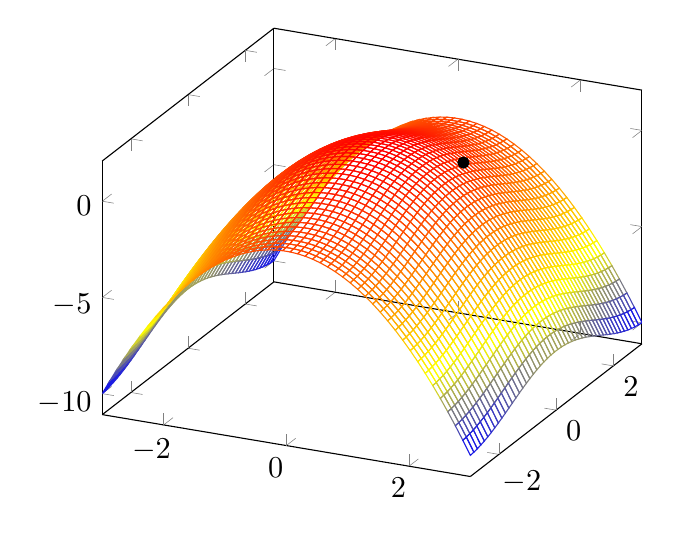
\begin{tikzpicture}
    \begin{axis}[]
        \addplot3[mesh, samples = 50, domain = -3:3]{cos(deg(y)) - x^2};
        \addplot3[black, mark=*] coordinates {(1, 1.047, -0.5)};
    \end{axis}
\end{tikzpicture}
    \caption{The surface $z = \cos{y} - x^2$}
    \label{fig:surface}
\end{figure}

We can see that $f(1, \pi/3) = -1/2$; therefore, the point $(1, \pi/3, -1/2)$ 
lies on the surface $z = \cos{y} - x^2$ (the black dot shown in figure \ref{
fig:surface}). If we fix $y$ such that $y = \pi/3$, we are looking at the 
intersection between the surface and the plane $y = \pi/3$ (see figure \ref{
fig:tangent}). 

\begin{figure}[htbp]
    \centering
    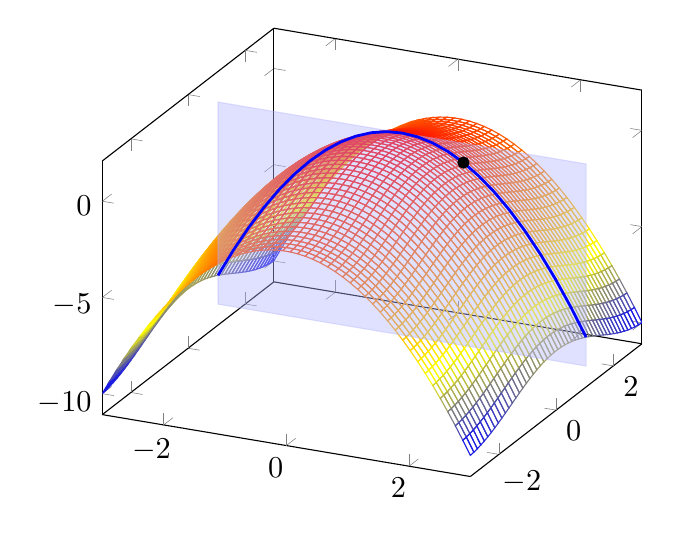
\begin{tikzpicture}
    \begin{axis}[]
        \addplot3[mesh, samples = 50, domain = -3:3]{cos(deg(y)) - x^2};
        \addplot3[black, mark=*] coordinates {(1, 1.047, -0.5)};
        \filldraw[blue!30, opacity = 0.4] (-3, 1.047, -10) -- (-3, 1.047, 0.5) 
        -- (3, 1.047, 0.5) -- (3, 1.047, -10) -- cycle;
        \addplot3+[draw=blue, line width = 1pt, domain = -3:3, samples y = 0, 
        mark=none] ({x}, 1.047, {0.5-x^2});
    \end{axis}
\end{tikzpicture}
    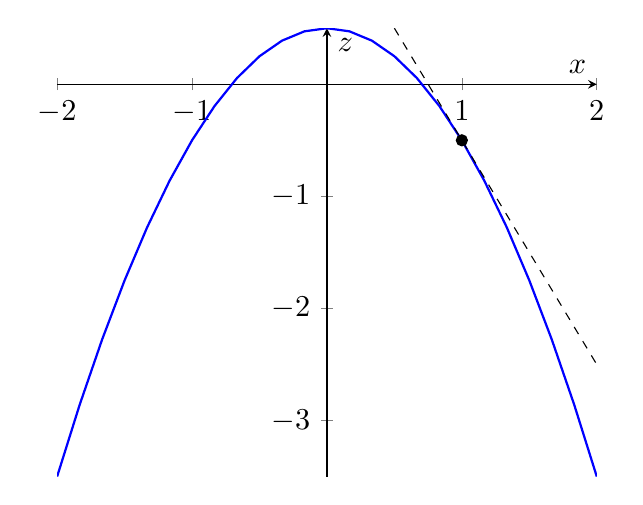
\begin{tikzpicture}
        \begin{axis}[axis lines = center, xlabel = $x$, ylabel = $z$]
            \addplot[blue, thick, domain = -2:2] {0.5-x^2};
            \addplot[black, thin, dashed, domain = 0.5:2] {-2*(x - 1) - 0.5};
            \addplot[black, mark=*] coordinates {(1, -0.5)};
        \end{axis}
    \end{tikzpicture}
    \caption{The intersection between the surface $z = \cos{y} - x^2$ and $y = 
    \pi/3$ is the parabola $z(x) = 1/2 - x^2$}
    \label{fig:tangent}
\end{figure}

We can describe this intersection as $g(x) = f(x, \pi/3)$, so the 
slope of a tangent line to this intersection is given by $g'(x) = f_x(x, 
\pi/3)$. This means, geometrically, $f_x(1, \pi/3)$ is the slope of the line 
that lies tangent to $z = f(x, y)$ at the point $(1, \pi/3, -1/2)$ and in the 
plane $y = \pi/3$ (see figure \ref{fig:tangent}). Alternatively, you could 
think of $f_x$ as the slope of the tangent line to the surface that is 
parallel to the $x$-axis. 

Similarly, we can fix $x = 1$ and look at the intersection between the surface 
$z = \cos{y} - x^2$ and the plane $x = 1$ (see figure \ref{fig:ytangent}. 
Just like before, we can describe this intersection as $h(y) = f(1, y)$, which 
means the slope of a line tangent to the intersection is given by $h'(y) = 
f_{y}(1, y)$. Therefore, as with $f_x$, $f_y(a, b)$ gives the slope of a line 
tangent to the point $\left(a, b, f(a, b) \right)$ and parallel to the $y$-axis. 

\begin{figure}[htbp]
    \centering
    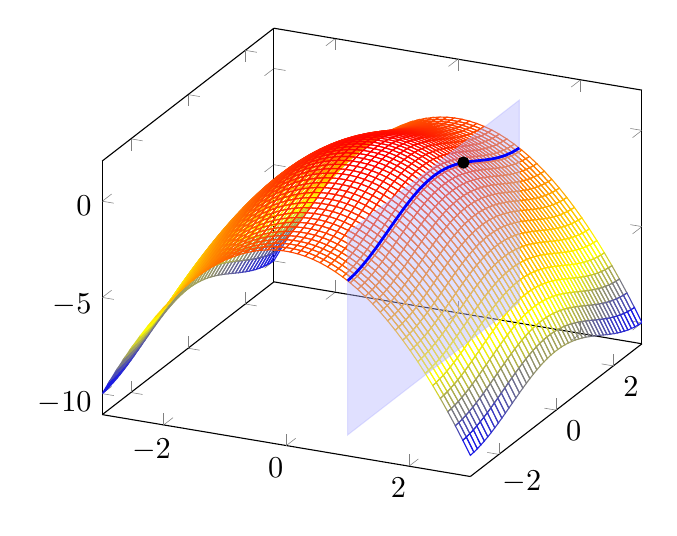
\begin{tikzpicture}
    \begin{axis}[]
        \addplot3[mesh, samples = 50, domain = -3:3]{cos(deg(y)) - x^2};
        \addplot3[black, mark=*] coordinates {(1, 1.047, -0.5)};
        \filldraw[blue!30, opacity = 0.4] (1, -3, -10) -- (1, -3, 0.5) 
        -- (1, 3, 0.5) -- (1, 3, -10) -- cycle;
        \addplot3+[draw=blue, line width = 1pt, domain = -3:3, samples y = 0, 
        mark=none] (1, {x}, {cos(deg(x))-1});
    \end{axis}
\end{tikzpicture}
    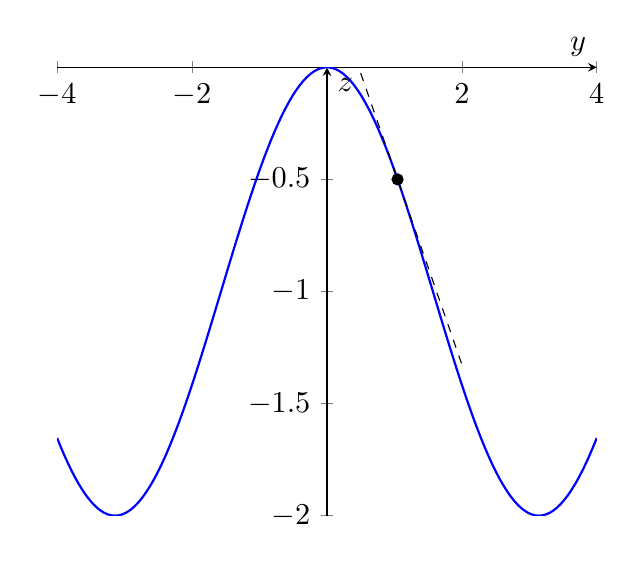
\begin{tikzpicture}
        \begin{axis}[axis lines = center, xlabel = $y$, ylabel = $z$]
            \addplot[blue, thick, domain = -4:4, samples = 150] 
            {cos(deg(x)) - 1};
            \addplot[black, thin, dashed, domain = 0.5:2] 
            {-0.866*(x - 1.047) - 0.5};
            \addplot[black, mark=*] coordinates {(1.047, -0.5)};
        \end{axis}
    \end{tikzpicture}
    \caption{The intersection between the surface $z = \cos{y} - x^2$ and 
    $x = 1$ is the trigonometric function $z = \cos{y} - 1$}
    \label{fig:ytangent}
\end{figure}

\textbf{Example}: The density of bacterial growth at a point $(x, y)$ on a 
flat agar plate is given by $D = 45/\left(2 + x^2 + y^2 \right)$. Find the 
rate of change of bacterial density at the point $(1, 3)$ (a) in the 
$x$-direction and (b) in the $y$-direction. Interpret the meaning of your 
results. 

\textbf{Solution}: The rate of change of a two-variable function in the 
$x$-direction is given by the partial derivative with respect to $x$:
$$D_x = \frac{\partial}{\partial x} \frac{45}{2 + x^2 + y^2} = \frac{-45 
\left( \partial/\partial x \right) \left(2 + x^2 + y^2 \right)}{\left(2 + 
x^2 + y^2 \right)^2}$$
$$= \frac{-90x}{\left( 2 + x^2 + y^2 \right)^2}$$

The rate of change in the $x$-direction at $(x, y) = (1, 3)$ is given by:
$$D_x(1, 3) = \frac{-90(1)}{\left( 2 + 1^2 + 3^2 \right)^2} = \frac{-90}{\left(
12 \right)^2} = \frac{-90}{144} = -\frac{5}{8}$$

This means that at $(1, 3)$, the density of bacteria is decreasing as you move 
away $x = 0$ along the line $y = 3$.

Similarly, the rate of change in the $y$-direction is given by the partial 
derivative with respect to $y$:
$$D_y = \frac{\partial}{\partial y} \frac{45}{2 + x^2 + y^2} = \frac{-45 \left(
\partial/\partial y \right) \left(2 + x^2 + y^2 \right)}{\left( 2 + x^2 + y^2 
\right)^2}$$
$$= \frac{-90y}{\left(2 + x^2 + y^2 \right)^2}$$

The rate of change in the $y$-direction at $(x, y) = (1, 3)$ is given by:
$$D_y(1, 3) = \frac{-90(3)}{\left(2 + 1^2 + 3^2 \right)^2} = \frac{-270}{144} 
= -\frac{15}{8}$$

This means that at $(1, 3)$ the density of bacteria is decreasing faster along 
the $y$-direction than along the $x$-direction. 

\begin{Exercise}[title = {Using partial derivatives to find tangent lines}, 
label = tangent]
Find equations for tangent lines to the surface at the given $xy$-coordinate. 
In which direction is the function changing the fastest?
\begin{enumerate}
\item $z = x^2e^{y/x}$, $(1, -1)$
\item $z = \cos{x} + y\sin{y}$, $(\pi, \pi/2)$
\item $z = x^2y - 3xy^2$, $(3, 2)$
\end{enumerate}
\vspace{75mm}
\end{Exercise}

\begin{Answer}[ref = tangent]
\begin{enumerate}
    \item $z(1, -1) = (1)^2e({-1/1} = 1/e$. Therefore, we are looking for 
    tangent lines through the point $(1, -1, 1/e)$. Finding a tangent line 
    parallel to the $x$-axis: $\frac{\partial z}{\partial x} = \frac{\partial}{
    \partial x} \left( x^2e^{y/x} \right) = x^2 \left( \frac{\partial}{\partial
    x}e^{y/x} \right) + e^{y/x} \left( \frac{\partial}{\partial x}x^2 \right) =
    x^2e^{y/x} \left( \frac{\partial}{\partial x} \frac{y}{x} \right) + 2x
    e^{y/x} = x^2 e^{y/x} \left( \frac{-y}{x^2} \right) + 2xe^{y/x} = \left( 
    2x - y \right)e^{y/x}$ and $z_x(1, -1) = \left( 2(1) - (-1) \right) 
    e^{-1/1} = \left(3 \right)e^{-1} = 3/e$. So, the slope of a line tangent to 
    the surface at $(1, -1, 1/e)$ parallel to the $x$-axis is $3/e$ and an 
    equation for that line is $z = 3/e \left(x - 1 \right) - 1/e$. 

    Finding a tangent line parallel to the $y$-axis: $\frac{\partial z}{
    \partial y} = \frac{\partial}{\partial y} \left( x^2e^{y/x} \right) = x
    e^{y/x}$ and $z_y(1, -1) = (1)e^{-1/1} = 1/e$. So, the slope of a line 
    tangent to the surface at $(1, -1, 1/e)$ parallel to the $y$-axis is $1/e$ 
    and an equation for that line is $z = 1/e \left(y + 1 \right) - 1/e$. 

    The function is changing faster in the $x$-direction. 

    \item $z(\pi, \pi/2) = \cos{(\pi)} + \frac{\pi}{2}\sin{(\pi/2)} = \frac{
    \pi}{2} - 1 $. Therefore, we are looking for tangent lines through the 
    point $(\pi, \pi/2, \pi/2 - 1)$. Finding a tangent line parallel to the 
    $x$-axis: $\frac{\partial z}{\partial x} = \frac{\partial}{\partial x} 
    \left( \cos{x} + y\sin{y} \right) = -\sin{x}$ and $z_x(\pi, \pi/2) = -\sin{
    \pi} = 0$. So, the slope of a line tangent to the surface at $(\pi, \pi/2, 
    \pi/2 - 1)$ parallel to the $x$-axis is $0$ and an equation for that line 
    is $z = \pi/2 - 1$.

    Finding a tangent line parallel to the $y$-axis: $\frac{\partial z}{
    \partial y} = \frac{\partial}{\partial y} \left( \cos{x} + y\sin{y} \right)
    = y \left( \frac{\partial}{\partial y}\sin{y} \right) + \sin{y} \left( 
    \frac{\partial}{\partial y} y \right) = y\cos{y} + \sin{y}$ and $z_y(\pi, 
    \pi/2) = \left( \frac{\pi}{2} \right) \cos{ \left( \frac{\pi}{2} \right) } 
    + \sin{ \left( \frac{\pi}{2} \right) } = 1$. So, the slope of a line tangent
    to the surface at $( \pi, \pi/2, \pi/2 - 1 )$ parallel to the $y$-axis is 
    $1$ and an equation for that line is $z = \left( y - \pi/2 \right) - \left(
    \pi/2 - 1 \right) = y - \pi + 1$. 

    The function is changing faster in the $y$-direction.

    \item $z(3, 2) = 3^2(2) - 3(3)(2^2) = 18 - 36 = -18$. Therefore, we are 
    looking for tangent lines through the point $(3, 2, -18)$. Finding a 
    tangent line parallel to the $x$-axis: $\frac{\partial z}{\partial x} = 
    \frac{\partial}{\partial x} \left( x^2y - 3xy^2 \right) = 2xy - 3y^2$ and 
    $z_x(3, 2) = 2(3)(2) - 3(2)^2 = 0$. So, the slope of a line tangent to the 
    surface at $(3, 2, -18)$ is $0$ and an equation for that line is $z = -18$

    Finding a tangent line parallel to the $y$-axis: $\frac{\partial z}{
    \partial y} = \frac{\partial}{\partial y} \left( x^2y - 3xy^2 \right) = 
    x^2 - 6xy$ and $z_y(3, 2) = 3^2 - 6(3)(2) = 9 - 36 = -27$. So, the slope of 
    a line tangent to the surface at $(3, 2, -18)$ is $-27$ and an equation for
    that line is $z = -27(y - 2) + -18 = -27y + 54 - 18 = 36 - 27y$.

    The function is changing faster in the $y$-direction. 
\end{enumerate}
\end{Answer}

\section{Gradient Vectors}
The gradient vector is used to find the direction of the maximum rate of change 
of a surface (for example, the steepest part of a mountain). In order to 
understand the gradient, we must first discuss directional derivatives. Recall 
that the partial derivatives, $f_x$ and $f_y$, can be used to define a plane 
tangent to the surface $z = f(x,y)$ (see figure \ref{fig:plane}). Directional 
derivatives allow us to find the slope of the tangent plane in directions 
other than the $x$- and $y$-directions. 

\begin{figure}[htbp]
    \centering
    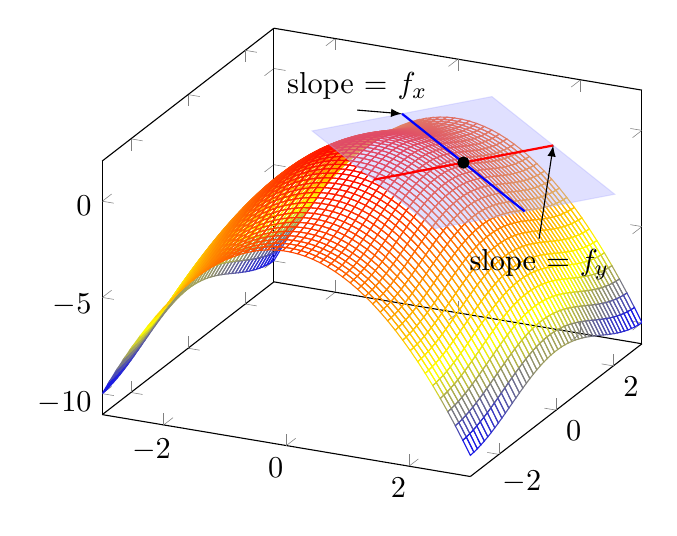
\begin{tikzpicture}
    \begin{axis}[]
        \addplot3[mesh, samples = 50, domain = -3:3]{cos(deg(y)) - x^2};
        \addplot3[black, mark=*] coordinates {(1, 1.047, -0.5)};
        \filldraw[blue!30, opacity = 0.4] (0, -2.094, 4.220) -- 
        (0, 4.189, -1.221) -- (2, 4.189, -5.221) -- (2, -2.094, 0.220) -- cycle;
        \draw[red, thick](1, -2.094, 2.220) -- (1, 4.189, -3.221);
        \draw[latex-] (0, 1.047, 1.5) -- (-0.5, 0.547, 2) node[above] {
        slope = $f_x$};
        \draw[blue, thick](0, 1.047, 1.5) -- (2, 1.047, -2.5);
        \draw[latex-](1, 4.189, -3.221) -- (2, 1.547, -4.5) node[below] {
        slope = $f_y$};
    \end{axis}
    \end{tikzpicture}
    \caption{The directional derivatives, $f_x$ and $f_y$ define a tangent 
    plane}
    \label{fig:plane}
\end{figure}

\subsection{Directional Derivatives}
<<<<<<< HEAD
The contour map in figure \ref{fig:mountain} shows the elevation, $f(x, y)$ 
=======
The contour map in figure \ref{fig:mountain} shows the elevation, $H(x, y)$, 
>>>>>>> 75c26aca4245f06f19f767709f3697abe6d41eba
for a mountain. You already know that you can use the partial derivatives, 
$f_x$ and $f_y$ to find the rate of change in elevation going east-west or 
north-south. But what about other directions? Suppose the hiking path you're 
on goes north-east. How can you predict the steepness (i.e. the rate of 
elevation change) along this path? The directional derivative allows us to 
find the rate of change in any direction. 

\begin{figure}[htbp]
    \centering
    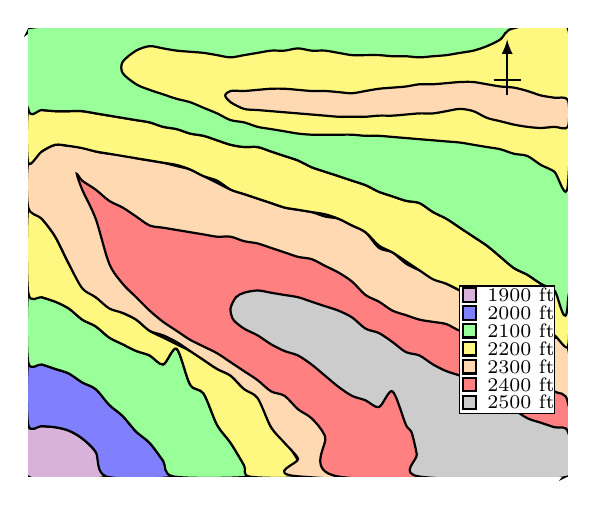
\begin{tikzpicture}
        \begin{axis}[xmin = 0, xmax = 20, ymin = 0, ymax = 20, ticks = none, 
        axis lines = center]
        \draw[fill = violet!30, draw = black, thick] plot[smooth cycle] 
        coordinates {(0, 2.3) (0.5, 2.25) (1, 2.2) (1.5, 2.05) (2, 1.7) 
        (2.5, 1.1) (2.9, 0) (0,0)};
        \draw[fill = blue!50, draw = black, thick] plot[smooth cycle] 
        coordinates {(0, 2.3) (0.5, 2.25) (1, 2.2) (1.5, 2.05) (2, 1.7) 
        (2.5, 1.1) (2.9, 0) (5.4, 0) (5, 0.7) (4.5, 1.5) (4, 2) (3.5, 2.7) 
        (3, 3.2) (2.5, 3.9) (2, 4.2) (1.5, 4.6) (1, 4.8) (0.5, 5) (0, 5.1)};
        \draw[fill = green!40, draw = black, thick] plot[smooth cycle] 
        coordinates {(5.4, 0) (5, 0.7) (4.5, 1.5) (4, 2) (3.5, 2.7) (3, 3.2) 
        (2.5, 3.9) (2, 4.2) (1.5, 4.6) (1, 4.8) (0.5, 5) (0, 5.1) (0, 8.2) 
        (0.5, 8) (1, 7.8) (1.5, 7.5) (2, 7) (2.5, 6.7) (3, 6.2) (3.5, 5.9) 
        (4, 5.6) (4.5, 5.4) (5, 5) (5.5, 5.7) (6, 4.1) (6.5, 3.7) (7, 2.3) 
        (7.5, 1.5) (8, 0.5) (8.2, 0)};
        \draw[fill = yellow!50, draw = black, thick] plot[smooth cycle] 
        coordinates {(0, 8.2) (0.5, 8) (1, 7.8) (1.5, 7.5) (2, 7) (2.5, 6.7) 
        (3, 6.2) (3.5, 5.9) (4, 5.6) (4.5, 5.4) (5, 5) (5.5, 5.7) (6, 4.1) 
        (6.5, 3.7) (7, 2.3) (7.5, 1.5) (8, 0.5) (8.2, 0) (10.1, 0) (10, 0.7) 
        (9.5, 1.6) (9, 2.2) (8.5, 3.6) (8, 3.9) (7.5, 4.5) (7, 4.8) (6.5, 5.2) 
        (6, 5.6) (5.5, 5.9) (5, 6.2) (4.5, 6.5) (4, 7) (3.5, 7.3) (3, 7.6) 
        (2.5, 8) (2, 8.5) (1.5, 9.5) (1, 10.7) (0.5, 11.5) (0, 12)};
        \draw[fill = orange!30, draw = black, thick] plot[smooth cycle] 
        coordinates {(20, 0) (10.1, 0) (10, 0.8) (9.5, 1.5) (9, 2.2) 
        (8.5, 3.5) (8, 3.9) (7.5, 4.5) (7, 4.8) (6.5, 5.2) (6, 5.6) (5.5, 6) 
        (5, 6.3) (4.5, 6.5) (4, 7) (3.5, 7.3) (3, 7.5) (2.5, 8) (2, 8.4) 
        (1.5, 9.5) (1, 10.7) (0.5, 11.5) (0, 12) (0, 14) (0.5, 14.5) (1, 14.8) 
        (1.5, 14.75) (2, 14.7) (2.5, 14.5) (3, 14.4) (3.5, 14.35) (4, 14.2) 
        (4.5, 14.1) (5, 14) (5.5, 13.85) (6, 13.7) (6.5, 13.4) (7, 13.1) 
        (7.5, 12.8) (8, 12.6) (8.5, 12.4) (9, 12.2) (9.5, 12) (10, 11.9) 
        (10.5, 11.8) (11, 11.6) (11.5, 11.5) (12, 11.2) (12.5, 10.9) 
        (13, 10.2) (13.5, 10) (14, 9.5) (14.5, 9.2) (15, 8.9) (15.5, 8.6) 
        (16, 8.3) (16.5, 8) (17, 7.6) (17.5, 7.4) (18, 7.2) (18.5, 6.9) 
        (19, 6.5) (19.5, 6.2) (20, 5.8)};
        \draw[fill = red!50, draw = black, thick] plot[smooth cycle] 
        coordinates {(20, 0) (11.5, 0) (11, 1.8) (10.5, 2.6) (10, 3) 
        (9.5, 3.6) (9, 3.8) (8.5, 4.3) (8, 4.7) (7.5, 5.1) (7, 5.5) (6.5, 5.8) 
        (6, 6.1) (5.5, 6.5) (5, 6.9) (4.5, 7.4) (4, 8) (3.5, 8.6) (3, 9.5) 
        (2.5, 11.5) (2, 12.8) (1.8, 13.5) (2, 13.2) (2.5, 12.8) (3, 12.3) 
        (3.5, 12) (4, 11.6) (4.5, 11.2) (5, 11.1) (5.5, 11) (6, 10.9) 
        (6.5, 10.8) (7, 10.7) (7.5, 10.7) (8, 10.5) (8.5, 10.4) (9, 10.2) 
        (9.5, 10) (10, 9.8) (10.5, 9.7) (11, 9.4) (11.5, 9.1) (12, 8.7) 
        (12.5, 8.1) (13, 7.8) (13.5, 7.4) (14, 7.2) (14.5, 7) (15, 6.9) 
        (15.5, 6.8) (16, 6.5) (16.5, 6.4) (17, 6) (17.5, 5.6) (18, 5.2) 
        (18.5, 4.8) (19, 4.3) (19.5, 3.8) (20, 3.3)};
        \draw[fill = gray!40, draw = black, thick] plot[smooth cycle] 
        coordinates {(14.5, 0) (14.4, 1) (14.2, 2) (14, 2.3) (13.5, 3.8) 
        (13, 3.1) (12.5, 3.4) (12, 3.6) (11.5, 4) (11, 4.5) (10.5, 5) 
        (10, 5.4) (9.5, 5.6) (9, 5.9) (8.5, 6.3) (8, 6.6) (7.6, 7) (7.5, 7.5) 
        (7.7, 8) (8, 8.2) (8.5, 8.3) (9, 8.2) (9.5, 8.1) (10, 8) (10.5, 7.8) 
        (11, 7.6) (11.5, 7.4) (12, 7.1) (12.5, 6.6) (13, 6.4) (13.5, 6) 
        (14, 5.55) (14.5, 5.4) (15, 5) (15.5, 4.7) (16, 4.5) (16.5, 4.2) 
        (17, 3.8) (17.5, 3.5) (18, 3) (18.5, 2.6) (19, 2.4) (19.5, 2.2) 
        (20, 2) (20, 0)};
        \draw[fill = yellow!50, draw = black, thick] plot[smooth cycle] 
        coordinates {(0, 14) (0.5, 14.5) (1, 14.8) (1.5, 14.75) (2, 14.65) 
        (2.5, 14.5) (3, 14.4) (3.5, 14.3) (4, 14.2) (4.5, 14.1) (5, 14) 
        (5.5, 13.9) (6, 13.7) (6.5, 13.4) (7, 13.2) (7.5, 12.8) (8, 12.6) 
        (8.5, 12.4) (9, 12.2) (9.5, 12) (10, 11.9) (10.5, 11.8) (11, 11.7) 
        (11.5, 11.5) (12, 11.2) (12.5, 10.9) (13, 10.3) (13.5, 10) (14, 9.6) 
        (14.5, 9.2) (15, 8.8) (15.5, 8.6) (16, 8.3) (16.5, 8) (17, 7.6) 
        (17.5, 7.4) (18, 7.2) (18.5, 6.9) (19, 6.5) (19.5, 6.3) (20, 5.8) 
        (20, 7.8) (19.5, 8.3) (19, 8.6) (18.5, 9) (18, 9.3) (17.5, 9.8) 
        (17, 10.3) (16.5, 10.7) (16, 11.1) (15.5, 11.5) (15, 11.8) 
        (14.5, 12.2) (14, 12.3) (13.5, 12.5) (13, 12.7) (12.5, 13) (12, 13.2) 
        (11.5, 13.4) (11, 13.6) (10.5, 13.8) (10, 14.1) (9.5, 14.3) (9, 14.5) 
        (8.5, 14.7) (8, 14.7) (7.5, 14.8) (7, 15) (6.5, 15.2) (6, 15.3) 
        (5.5, 15.5) (5, 15.6) (4.5, 15.8) (4, 15.9) (3.5, 16) (3, 16.1) 
        (2.5, 16.2) (2, 16.3) (1.5, 16.3) (1, 16.3) (0.5, 16.35) (0, 16.4)};
        \draw[fill = green!40, draw = black, thick] plot[smooth cycle] 
        coordinates {(20, 7.8) (19.5, 8.3) (19, 8.6) (18.5, 9) (18, 9.3) 
        (17.5, 9.8) (17, 10.3) (16.5, 10.7) (16, 11.1) (15.5, 11.5) (15, 11.8) 
        (14.5, 12.2) (14, 12.3) (13.5, 12.5) (13, 12.7) (12.5, 13) (12, 13.2) 
        (11.5, 13.4) (11, 13.6) (10.5, 13.8) (10, 14.1) (9.5, 14.3) (9, 14.5) 
        (8.5, 14.7) (8, 14.7) (7.5, 14.8) (7, 15) (6.5, 15.2) (6, 15.3) 
        (5.5, 15.5) (5, 15.6) (4.5, 15.8) (4, 15.9) (3.5, 16) (3, 16.1) 
        (2.5, 16.2) (2, 16.3) (1.5, 16.3) (1, 16.3) (0.5, 16.35) (0, 16.4) 
        (0, 20) (20, 20)};
        \draw[fill = yellow!50, draw = black, thick] plot[smooth cycle] 
        coordinates {(20, 13) (19.5, 13.6) (19, 13.9) (18.5, 14.3) (18, 14.4) 
        (17.5, 14.6) (17, 14.7) (16.5, 14.8) (16, 14.9) (15.5, 14.95) (15, 15) 
        (14.5, 15.05) (14, 15.1) (13.5, 15.15) (13, 15.2) (12.5, 15.2) 
        (12, 15.25) (11.5, 15.25) (11, 15.25) (10.5, 15.25) (10, 15.3) 
        (9.5, 15.4) (9, 15.5) (8.5, 15.6) (8, 15.8) (7.5, 15.9) (7, 16.2) 
        (6.5, 16.45) (6, 16.7) (5.5, 16.85) (5, 17.05) (4.5, 17.25) (4, 17.5) 
        (3.5, 18) (3.5, 18.5) (4, 19) (4.5, 19.2) (5, 19.1) (5.5, 19) 
        (6, 18.95) (6.5, 18.9) (7, 18.8) (7.5, 18.7) (8, 18.8) (8.5, 18.9) 
        (9, 19) (9.5, 19) (10, 19.1) (10.5, 19) (11, 19) (11.5, 18.9) 
        (12, 18.8) (12.5, 18.8) (13, 18.8) (13.5, 18.75) (14, 18.75) 
        (14.5, 18.7) (15, 18.75) (15.5, 18.8) (16, 18.9) (16.5, 19) 
        (17, 19.2) (17.5, 19.5) (18, 20) (20, 20)};
        \draw[fill = orange!30, draw = black, thick] plot[smooth cycle] 
        coordinates {(20, 15.6) (19.5, 15.6) (19, 15.55) (18.5, 15.6) 
        (18, 15.7) (17.5, 15.85) (17, 16) (16.5, 16.3) (16, 16.4) (15.5, 16.3) 
        (15, 16.2) (14.5, 16.2) (14, 16.15) (13.5, 16.1) (13, 16.1) 
        (12.5, 16.05) (12, 16.05) (11.5, 16.05) (11, 16.1) (10.5, 16.15) 
        (10, 16.2) (9.5, 16.25) (9, 16.3) (8.5, 16.35) (8, 16.4) (7.5, 16.7) 
        (7.3, 17) (7.5, 17.2) (8, 17.2) (8.5, 17.25) (9, 17.3) (9.5, 17.3) 
        (10, 17.25) (10.5, 17.2) (11, 17.2) (11.5, 17.15) (12, 17.1) 
        (12.5, 17.2) (13, 17.3) (13.5, 17.35) (14, 17.4) (14.5, 17.5) 
        (15, 17.5) (15.5, 17.55) (16, 17.6) (16.5, 17.6) (17, 17.5) 
        (17.5, 17.4) (18, 17.35) (18.5, 17.2) (19, 17) (19.5, 16.9) 
        (20, 16.8)};
        \draw[fill = white, draw = black] (19.5, 2.8) rectangle (16, 8.5);
        \draw[fill = violet!30, draw = black, thick] (16.1, 8.4) rectangle 
        (16.6, 7.8) node[right, font = \scriptsize, yshift = 0.09cm] {1900 ft};
        \draw[fill = blue!50, draw = black, thick] (16.1, 7.6) rectangle 
        (16.6, 7) node[right, font = \scriptsize, yshift = 0.09cm] {2000 ft};
        \draw[fill = green!40, draw = black, thick] (16.1, 6.8) rectangle 
        (16.6, 6.2) node[right, font = \scriptsize, yshift = 0.09cm] {2100 ft};
        \draw[fill = yellow!50, draw = black, thick] (16.1, 6) rectangle 
        (16.6, 5.4) node[right, font = \scriptsize, yshift = 0.09cm] {2200 ft};
        \draw[fill = orange!30, draw = black, thick] (16.1, 5.2) rectangle 
        (16.6, 4.6) node[right, font = \scriptsize, yshift = 0.09cm] {2300 ft};
        \draw[fill = red!50, draw = black, thick] (16.1, 4.4) rectangle 
        (16.6, 3.8) node[right, font = \scriptsize, yshift = 0.09cm] {2400 ft};
        \draw[fill = gray!40, draw = black, thick] (16.1, 3.6) rectangle 
        (16.6, 3) node[right, font = \scriptsize, yshift = 0.09cm] {2500 ft};
        \draw[-latex, black, thick] (17.75, 17) -- (17.75, 19.5);
        \draw[black, thick] (17.25, 17.7) -- (18.25, 17.7);
        \end{axis}
    \end{tikzpicture}
    \caption{The contour plot shows the elevation of a mountain. $f_x$ gives 
    the slope going east, while $f_y$ gives the slope going north}
    \label{fig:mountain}
\end{figure}

At some point, $(x_o, y_o)$, the partial derivatives $f_x(x_o, y_o)$ and 
$f_y(x_o, y_o)$ give the rate of change of elevation in the east-west and 
north-south directions, respectively (see figure \ref{fig:mount_deriv}). 

\begin{figure}[htbp]
    \centering
    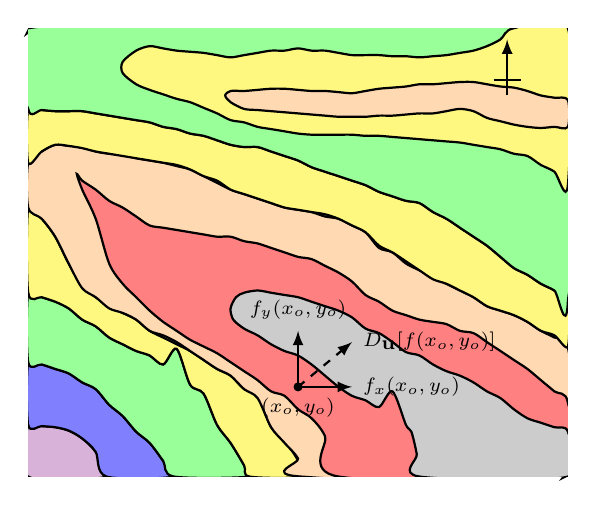
\begin{tikzpicture}
        \begin{axis}[xmin = 0, xmax = 20, ymin = 0, ymax = 20, ticks = none, 
        axis lines = center]
        \draw[fill = violet!30, draw = black, thick] plot[smooth cycle] 
        coordinates {(0, 2.3) (0.5, 2.25) (1, 2.2) (1.5, 2.05) (2, 1.7) 
        (2.5, 1.1) (2.9, 0) (0,0)};
        \draw[fill = blue!50, draw = black, thick] plot[smooth cycle] 
        coordinates {(0, 2.3) (0.5, 2.25) (1, 2.2) (1.5, 2.05) (2, 1.7) 
        (2.5, 1.1) (2.9, 0) (5.4, 0) (5, 0.7) (4.5, 1.5) (4, 2) (3.5, 2.7) 
        (3, 3.2) (2.5, 3.9) (2, 4.2) (1.5, 4.6) (1, 4.8) (0.5, 5) (0, 5.1)};
        \draw[fill = green!40, draw = black, thick] plot[smooth cycle] 
        coordinates {(5.4, 0) (5, 0.7) (4.5, 1.5) (4, 2) (3.5, 2.7) (3, 3.2) 
        (2.5, 3.9) (2, 4.2) (1.5, 4.6) (1, 4.8) (0.5, 5) (0, 5.1) (0, 8.2) 
        (0.5, 8) (1, 7.8) (1.5, 7.5) (2, 7) (2.5, 6.7) (3, 6.2) (3.5, 5.9) 
        (4, 5.6) (4.5, 5.4) (5, 5) (5.5, 5.7) (6, 4.1) (6.5, 3.7) (7, 2.3) 
        (7.5, 1.5) (8, 0.5) (8.2, 0)};
        \draw[fill = yellow!50, draw = black, thick] plot[smooth cycle] 
        coordinates {(0, 8.2) (0.5, 8) (1, 7.8) (1.5, 7.5) (2, 7) (2.5, 6.7) 
        (3, 6.2) (3.5, 5.9) (4, 5.6) (4.5, 5.4) (5, 5) (5.5, 5.7) (6, 4.1) 
        (6.5, 3.7) (7, 2.3) (7.5, 1.5) (8, 0.5) (8.2, 0) (10.1, 0) (10, 0.7) 
        (9.5, 1.6) (9, 2.2) (8.5, 3.6) (8, 3.9) (7.5, 4.5) (7, 4.8) (6.5, 5.2) 
        (6, 5.6) (5.5, 5.9) (5, 6.2) (4.5, 6.5) (4, 7) (3.5, 7.3) (3, 7.6) 
        (2.5, 8) (2, 8.5) (1.5, 9.5) (1, 10.7) (0.5, 11.5) (0, 12)};
        \draw[fill = orange!30, draw = black, thick] plot[smooth cycle] 
        coordinates {(20, 0) (10.1, 0) (10, 0.8) (9.5, 1.5) (9, 2.2) 
        (8.5, 3.5) (8, 3.9) (7.5, 4.5) (7, 4.8) (6.5, 5.2) (6, 5.6) (5.5, 6) 
        (5, 6.3) (4.5, 6.5) (4, 7) (3.5, 7.3) (3, 7.5) (2.5, 8) (2, 8.4) 
        (1.5, 9.5) (1, 10.7) (0.5, 11.5) (0, 12) (0, 14) (0.5, 14.5) (1, 14.8) 
        (1.5, 14.75) (2, 14.7) (2.5, 14.5) (3, 14.4) (3.5, 14.35) (4, 14.2) 
        (4.5, 14.1) (5, 14) (5.5, 13.85) (6, 13.7) (6.5, 13.4) (7, 13.1) 
        (7.5, 12.8) (8, 12.6) (8.5, 12.4) (9, 12.2) (9.5, 12) (10, 11.9) 
        (10.5, 11.8) (11, 11.6) (11.5, 11.5) (12, 11.2) (12.5, 10.9) 
        (13, 10.2) (13.5, 10) (14, 9.5) (14.5, 9.2) (15, 8.9) (15.5, 8.6) 
        (16, 8.3) (16.5, 8) (17, 7.6) (17.5, 7.4) (18, 7.2) (18.5, 6.9) 
        (19, 6.5) (19.5, 6.2) (20, 5.8)};
        \draw[fill = red!50, draw = black, thick] plot[smooth cycle] 
        coordinates {(20, 0) (11.5, 0) (11, 1.8) (10.5, 2.6) (10, 3) 
        (9.5, 3.6) (9, 3.8) (8.5, 4.3) (8, 4.7) (7.5, 5.1) (7, 5.5) (6.5, 5.8) 
        (6, 6.1) (5.5, 6.5) (5, 6.9) (4.5, 7.4) (4, 8) (3.5, 8.6) (3, 9.5) 
        (2.5, 11.5) (2, 12.8) (1.8, 13.5) (2, 13.2) (2.5, 12.8) (3, 12.3) 
        (3.5, 12) (4, 11.6) (4.5, 11.2) (5, 11.1) (5.5, 11) (6, 10.9) 
        (6.5, 10.8) (7, 10.7) (7.5, 10.7) (8, 10.5) (8.5, 10.4) (9, 10.2) 
        (9.5, 10) (10, 9.8) (10.5, 9.7) (11, 9.4) (11.5, 9.1) (12, 8.7) 
        (12.5, 8.1) (13, 7.8) (13.5, 7.4) (14, 7.2) (14.5, 7) (15, 6.9) 
        (15.5, 6.8) (16, 6.5) (16.5, 6.4) (17, 6) (17.5, 5.6) (18, 5.2) 
        (18.5, 4.8) (19, 4.3) (19.5, 3.8) (20, 3.3)};
        \draw[fill = gray!40, draw = black, thick] plot[smooth cycle] 
        coordinates {(14.5, 0) (14.4, 1) (14.2, 2) (14, 2.3) (13.5, 3.8) 
        (13, 3.1) (12.5, 3.4) (12, 3.6) (11.5, 4) (11, 4.5) (10.5, 5) 
        (10, 5.4) (9.5, 5.6) (9, 5.9) (8.5, 6.3) (8, 6.6) (7.6, 7) (7.5, 7.5) 
        (7.7, 8) (8, 8.2) (8.5, 8.3) (9, 8.2) (9.5, 8.1) (10, 8) (10.5, 7.8) 
        (11, 7.6) (11.5, 7.4) (12, 7.1) (12.5, 6.6) (13, 6.4) (13.5, 6) 
        (14, 5.55) (14.5, 5.4) (15, 5) (15.5, 4.7) (16, 4.5) (16.5, 4.2) 
        (17, 3.8) (17.5, 3.5) (18, 3) (18.5, 2.6) (19, 2.4) (19.5, 2.2) 
        (20, 2) (20, 0)};
        \draw[fill = yellow!50, draw = black, thick] plot[smooth cycle] 
        coordinates {(0, 14) (0.5, 14.5) (1, 14.8) (1.5, 14.75) (2, 14.65) 
        (2.5, 14.5) (3, 14.4) (3.5, 14.3) (4, 14.2) (4.5, 14.1) (5, 14) 
        (5.5, 13.9) (6, 13.7) (6.5, 13.4) (7, 13.2) (7.5, 12.8) (8, 12.6) 
        (8.5, 12.4) (9, 12.2) (9.5, 12) (10, 11.9) (10.5, 11.8) (11, 11.7) 
        (11.5, 11.5) (12, 11.2) (12.5, 10.9) (13, 10.3) (13.5, 10) (14, 9.6) 
        (14.5, 9.2) (15, 8.8) (15.5, 8.6) (16, 8.3) (16.5, 8) (17, 7.6) 
        (17.5, 7.4) (18, 7.2) (18.5, 6.9) (19, 6.5) (19.5, 6.3) (20, 5.8) 
        (20, 7.8) (19.5, 8.3) (19, 8.6) (18.5, 9) (18, 9.3) (17.5, 9.8) 
        (17, 10.3) (16.5, 10.7) (16, 11.1) (15.5, 11.5) (15, 11.8) 
        (14.5, 12.2) (14, 12.3) (13.5, 12.5) (13, 12.7) (12.5, 13) (12, 13.2) 
        (11.5, 13.4) (11, 13.6) (10.5, 13.8) (10, 14.1) (9.5, 14.3) (9, 14.5) 
        (8.5, 14.7) (8, 14.7) (7.5, 14.8) (7, 15) (6.5, 15.2) (6, 15.3) 
        (5.5, 15.5) (5, 15.6) (4.5, 15.8) (4, 15.9) (3.5, 16) (3, 16.1) 
        (2.5, 16.2) (2, 16.3) (1.5, 16.3) (1, 16.3) (0.5, 16.35) (0, 16.4)};
        \draw[fill = green!40, draw = black, thick] plot[smooth cycle] 
        coordinates {(20, 7.8) (19.5, 8.3) (19, 8.6) (18.5, 9) (18, 9.3) 
        (17.5, 9.8) (17, 10.3) (16.5, 10.7) (16, 11.1) (15.5, 11.5) (15, 11.8) 
        (14.5, 12.2) (14, 12.3) (13.5, 12.5) (13, 12.7) (12.5, 13) (12, 13.2) 
        (11.5, 13.4) (11, 13.6) (10.5, 13.8) (10, 14.1) (9.5, 14.3) (9, 14.5) 
        (8.5, 14.7) (8, 14.7) (7.5, 14.8) (7, 15) (6.5, 15.2) (6, 15.3) 
        (5.5, 15.5) (5, 15.6) (4.5, 15.8) (4, 15.9) (3.5, 16) (3, 16.1) 
        (2.5, 16.2) (2, 16.3) (1.5, 16.3) (1, 16.3) (0.5, 16.35) (0, 16.4) 
        (0, 20) (20, 20)};
        \draw[fill = yellow!50, draw = black, thick] plot[smooth cycle] 
        coordinates {(20, 13) (19.5, 13.6) (19, 13.9) (18.5, 14.3) (18, 14.4) 
        (17.5, 14.6) (17, 14.7) (16.5, 14.8) (16, 14.9) (15.5, 14.95) (15, 15) 
        (14.5, 15.05) (14, 15.1) (13.5, 15.15) (13, 15.2) (12.5, 15.2) 
        (12, 15.25) (11.5, 15.25) (11, 15.25) (10.5, 15.25) (10, 15.3) 
        (9.5, 15.4) (9, 15.5) (8.5, 15.6) (8, 15.8) (7.5, 15.9) (7, 16.2) 
        (6.5, 16.45) (6, 16.7) (5.5, 16.85) (5, 17.05) (4.5, 17.25) (4, 17.5) 
        (3.5, 18) (3.5, 18.5) (4, 19) (4.5, 19.2) (5, 19.1) (5.5, 19) 
        (6, 18.95) (6.5, 18.9) (7, 18.8) (7.5, 18.7) (8, 18.8) (8.5, 18.9) 
        (9, 19) (9.5, 19) (10, 19.1) (10.5, 19) (11, 19) (11.5, 18.9) 
        (12, 18.8) (12.5, 18.8) (13, 18.8) (13.5, 18.75) (14, 18.75) 
        (14.5, 18.7) (15, 18.75) (15.5, 18.8) (16, 18.9) (16.5, 19) (17, 19.2) 
        (17.5, 19.5) (18, 20) (20, 20)};
        \draw[fill = orange!30, draw = black, thick] plot[smooth cycle] 
        coordinates {(20, 15.6) (19.5, 15.6) (19, 15.55) (18.5, 15.6) 
        (18, 15.7) (17.5, 15.85) (17, 16) (16.5, 16.3) (16, 16.4) (15.5, 16.3) 
        (15, 16.2) (14.5, 16.2) (14, 16.15) (13.5, 16.1) (13, 16.1) 
        (12.5, 16.05) (12, 16.05) (11.5, 16.05) (11, 16.1) (10.5, 16.15) 
        (10, 16.2) (9.5, 16.25) (9, 16.3) (8.5, 16.35) (8, 16.4) (7.5, 16.7) 
        (7.3, 17) (7.5, 17.2) (8, 17.2) (8.5, 17.25) (9, 17.3) (9.5, 17.3) 
        (10, 17.25) (10.5, 17.2) (11, 17.2) (11.5, 17.15) (12, 17.1) 
        (12.5, 17.2) (13, 17.3) (13.5, 17.35) (14, 17.4) (14.5, 17.5) 
        (15, 17.5) (15.5, 17.55) (16, 17.6) (16.5, 17.6) (17, 17.5) 
        (17.5, 17.4) (18, 17.35) (18.5, 17.2) (19, 17) (19.5, 16.9) 
        (20, 16.8)};
        \draw[black, fill = black] (10, 4) circle (0.5mm) node[below, 
        font = \scriptsize] {$(x_o, y_o)$};
        \draw[black, thick, -latex] (10, 4) -- (10, 6.5) node[above, 
        font = \scriptsize] {$f_y(x_o, y_o)$}; 
        \draw[black, thick, -latex] (10, 4) -- (12, 4) node[right, 
        font = \scriptsize] {$f_x(x_o, y_o)$};
        \draw[black, thick, dashed, -latex] (10, 4) -- (12, 6) node[right, 
        font = \scriptsize] {$D_{\textbf{u}} [f(x_o, y_o)]$};
        \draw[-latex, black, thick] (17.75, 17) -- (17.75, 19.5);
        \draw[black, thick] (17.25, 17.7) -- (18.25, 17.7);
        \end{axis}
    \end{tikzpicture}
    \caption{If \textbf{u} points north-east, then the directional derivative 
    of $f(x, y)$ at $(x_o, y_o)$, $D_{\textbf{u}} \left[ f(x_o, y_o ) 
    \right]$, tells the rate of change going north-east}
    \label{fig:mount_deriv}
\end{figure}

To find the rate of change at $(x_o, y_o)$, in the direction of some arbitrary 
unit vector, $\textbf{u} = \left[ a, b \right] = a\textbf{i} + b\textbf{j}$, 
we first note that the point $Q = (x_o, y_o, z_o)$, where $z_o = f(x_o, y_o)$, 
lies on the surface defined by $z = f(x, y)$. There is a vertical plane, $P$, 
that passes through $Q$ and points in the direction of \textbf{u}. This 
intersection defines curve $C$, which lies on the surface, and the slope of 
this curve at $Q = (x_o, y_o, z_o)$ is the directional derivative of $H$ in 
the direction of \textbf{u} (see figure \ref{fig:direct_deriv}). 

\begin{figure}[htbp]
    \centering
    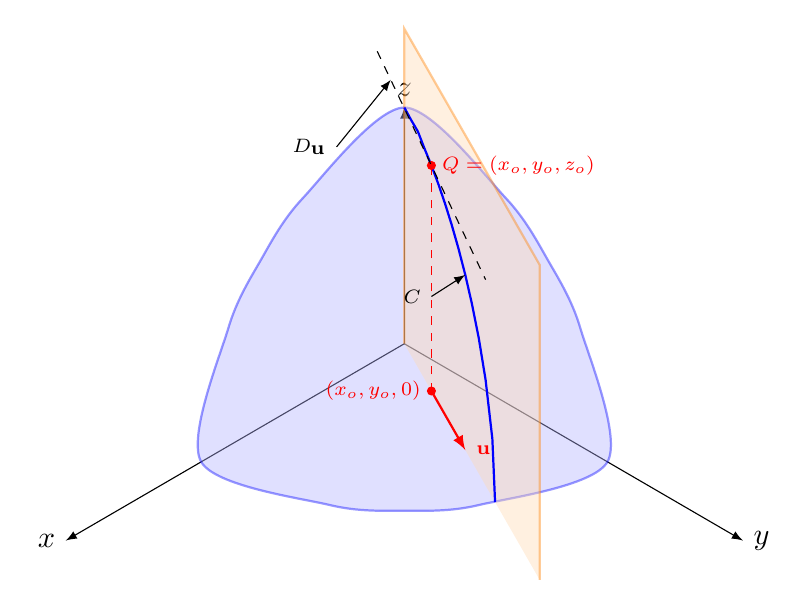
\begin{tikzpicture}[x = {(-0.86cm, -0.5cm)}, y = {(0.86cm, -0.5cm)}, 
    z = {(0cm, 1cm)}]
        \draw[-latex] (0,0,0) -- (5,0,0) node[left] {$x$};
        \draw[-latex] (0,0,0) -- (0,5,0) node[right] {$y$};
        \draw[-latex] (0,0,0) -- (0,0,3) node[above] {$z$};
        \draw[blue, thick, fill = blue!30, opacity = 0.4] plot[smooth cycle] 
        coordinates {(3, 0, 0) (2.598, 0, 1.5) (2.121, 0, 2.121) 
        (1.5, 0, 2.598) (0, 0, 3) (0, 1.5, 2.598) (0, 2.121, 2.121) 
        (0, 2.598, 1.5) (0, 3, 0) (1.5, 2.598, 0) (2.121, 2.121, 0) 
        (2.598, 1.5, 0)};
        \draw[orange, thick, fill = orange!30, opacity = 0.4] (0, 0, 0) -- 
        (0, 0, 4) -- (2, 4, 4) -- (2, 4, 0);
        \draw[red, thick, -latex] (0.4, 0.8, 0) -- (0.9, 1.8, 0) 
        node[right, font = \scriptsize] {\textbf{u}};
        \draw[blue, thick] (0,0,3) -- (0.1, 0.2, 2.992) -- (0.2, 0.4, 2.996) 
        -- (0.3, 0.6, 2.924) -- (0.4, 0.8, 2.864) -- (0.5, 1, 2.784) -- 
        (0.6, 1.2, 2.683) -- (0.7, 1.4, 2.559) -- (0.8, 1.6, 2.408) -- 
        (0.9, 1.8, 2.225) -- (1, 2, 2) -- (1.1, 2.2, 1.718) -- 
        (1.2, 2.4, 1.342) -- (1.3, 2.6, 0.742) -- (1.34, 2.68, 0);
        \draw[latex-] (0.9, 1.8, 2.225) -- (1.2, 1.6, 2) 
        node[left, font = \scriptsize] {$C$};
        \draw[red, dashed] (0.4, 0.8, 0) -- (0.4, 0.8, 2.864);
        \draw[red, fill = red] (0.4, 0.8, 2.864) circle (0.5mm) 
        node[right, font = \scriptsize] {$Q = (x_o, y_o, z_o)$};
        \draw[red, fill = red] (0.4, 0.8, 0) circle (0.5mm) 
        node[left, font = \scriptsize] {$(x_o, y_o, 0)$};
        \draw[black, dashed] (-0.4, -0.8, 3.11384) -- (1.2, 2.4, 2.6142);
        \draw[latex-] (-0.2, -0.4, 3.0514) -- (1, 0, 3) 
        node[left, font = \scriptsize] {$D_{\textbf{u}}$}; 
    \end{tikzpicture}
    \caption{The slope of the curve formed between the plane parallel to 
    \textbf{u} and the surface $z = f(x, y)$ is the directional derivative, 
    $D_{\textbf{u}}$}
    \label{fig:direct_deriv}
\end{figure}

We can choose another point, $R = (x, y, z)$, the is $h$ units away from $Q$ 
along \textbf{u} (see \ref{fig:direct_deriv2}). Then the change in $x$ is $x - 
x_o = ha$ and the change is $y$ is $y - y_o = hb$. And the slope from $Q$ to 
$R$ is given by:
$$\frac{\delta z}{h} = \frac{f(x, y) - f(x_o, y_o)}{h}$$

\begin{figure}[htbp]
    \centering
    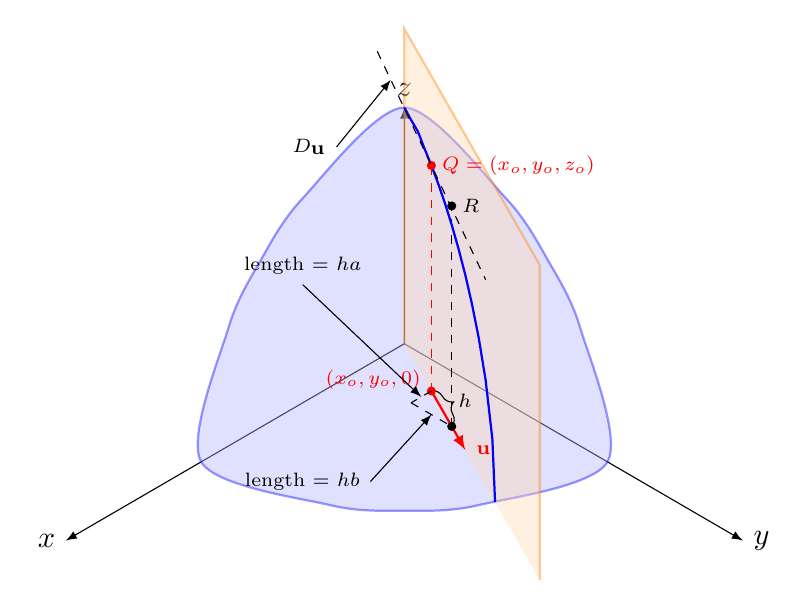
\begin{tikzpicture}[x = {(-0.86cm, -0.5cm)}, y = {(0.86cm, -0.5cm)}, 
    z = {(0cm, 1cm)}]
        \draw[-latex] (0,0,0) -- (5,0,0) node[left] {$x$};
        \draw[-latex] (0,0,0) -- (0,5,0) node[right] {$y$};
        \draw[-latex] (0,0,0) -- (0,0,3) node[above] {$z$};
        \draw[blue, thick, fill = blue!30, opacity = 0.4] plot[smooth cycle] 
        coordinates {(3, 0, 0) (2.598, 0, 1.5) (2.121, 0, 2.121) 
        (1.5, 0, 2.598) (0, 0, 3) (0, 1.5, 2.598) (0, 2.121, 2.121) 
        (0, 2.598, 1.5) (0, 3, 0) (1.5, 2.598, 0) (2.121, 2.121, 0) 
        (2.598, 1.5, 0)};
        \draw[orange, thick, fill = orange!30, opacity = 0.4] (0, 0, 0) -- 
        (0, 0, 4) -- (2, 4, 4) -- (2, 4, 0);
        \draw[red, thick, -latex] (0.4, 0.8, 0) -- (0.9, 1.8, 0) 
        node[right, font = \scriptsize] {\textbf{u}};
        \draw[black, fill = black] (0.7, 1.4, 0) circle (0.5mm);
        \draw[decorate, decoration = {brace, amplitude = 5pt}] (0.4, 0.8, 0) 
        -- (0.7, 1.4, 0) node[midway, xshift = 0.3cm, yshift = 0.1cm, 
        font = \scriptsize] {$h$};
        \draw[dashed] (0.7, 1.4, 0) -- (0.7, 1.4, 2.8);
        \draw[black, fill = black] (0.7, 1.4, 2.8) circle (0.5mm) node[right, 
        font = \scriptsize] {$R$};
        \draw[blue, thick] (0,0,3) -- (0.1, 0.2, 2.992) -- (0.2, 0.4, 2.996) 
        -- (0.3, 0.6, 2.924) -- (0.4, 0.8, 2.864) -- (0.5, 1, 2.784) -- 
        (0.6, 1.2, 2.683) -- (0.7, 1.4, 2.559) -- (0.8, 1.6, 2.408) -- 
        (0.9, 1.8, 2.225) -- (1, 2, 2) -- (1.1, 2.2, 1.718) -- 
        (1.2, 2.4, 1.342) -- (1.3, 2.6, 0.742) -- (1.34, 2.68, 0);
        \draw[red, dashed] (0.4, 0.8, 0) -- (0.4, 0.8, 2.864);
        \draw[red, fill = red] (0.4, 0.8, 2.864) circle (0.5mm) 
        node[right, font = \scriptsize] {$Q = (x_o, y_o, z_o)$};
        \draw[red, fill = red] (0.4, 0.8, 0) circle (0.5mm) 
        node[left, font = \scriptsize, yshift = 0.15cm] {$(x_o, y_o, 0)$};
        \draw[black, dashed] (-0.4, -0.8, 3.11384) -- (1.2, 2.4, 2.6142);
        \draw[latex-] (-0.2, -0.4, 3.0514) -- (1, 0, 3) 
        node[left, font = \scriptsize] {$D_{\textbf{u}}$}; 
        \draw[dashed] (0.4, 0.8, 0) -- (0.7, 0.8, 0);
        \draw[dashed] (0.7, 0.8, 0) -- (0.7, 1.4, 0);
        \draw[latex-] (0.7, 1.1, 0) -- (2, 1.5, 0) node[left, font = 
        \scriptsize] {length = $hb$};
        \draw[latex-] (0.55, 0.8, 0) -- (1.5, 0, 1.5) node[above, font = 
        \scriptsize] {length = $ha$};
    \end{tikzpicture}
    \caption{A second point, $R$, along \textbf{u} is $h$ units away along 
    \textbf{u}}
    \label{fig:direct_deriv2}
\end{figure}

We find the directional derivative by substituting for $x$ and $y$ and taking 
the limit as $h$ goes to zero:
$$D_{\textbf{u}} f(x_0, y_0) = \lim_{h \to 0} \frac{f(x_o + ha, y_o + hb) - 
f(x_o, y_o)}{h}$$

How is this related to $f_x$ and $f_y$? Let's define $g(h)$ such that $g(h) = 
f(x_o + ha, y_o + hb)$. Then
$$g'(0) = \lim_{h \to 0} \frac{g(h) - g(0)}{h}$$
$$= \lim_{h \to 0} = \frac{f(x_o + ha, y_o + hb) - f(x_o, y_o)}{h} = 
D_{\textbf{u}} f(x_o, y_o)$$

We can also apply the Chain Rule to $g(h)$:
$$g'(h) = \frac{\partial f}{\partial x} \frac{dx}{dh} + \frac{\partial f}{
\partial y} \frac{dy}{dh} = f_x(x, y)a + f_y(x, y)b$$

Substituting $h = 0$, $x = x_o$, and $y = y_o$, we see that:
$$g'(0) = f_x(x_o, y_o)a + f_y(x_o, y_o)b$$

Which means that:
$$D_{\textbf{u}} f(x_o, y_o) = f_x(x_o, y_o)a + f_y(x_o, y_o)b$$

So a directional derivative is:

\begin{mdframed}[style = important, frametitle = {The Directional Derivative}]
Let $f$ be a differentiable function and \textbf{u} be a unit vector, 
<<<<<<< HEAD
$\textbf{u} = \left[ a, b \right]$. Then the directional derivative in the 
direction of \textbf{u} is:
$$D_{\textbf{u}} f(x, y) = f_x(x, y)a + f_y(x, y)b = \textbf{u}_x \left[ 
\frac{\partial}{\partial x} f(x, y) \right] + \textbf{u}_y \left[ \frac{
\partial}{\partial y} f(x, y) \right]$$
=======
$\textbf{u} = \left[ a, b \right]$. This means the directional derivative in the direction of 
\textbf{u} is:
$$D_u f(x, y) = f_x(x, y)a + f_y(x, y)b = \textbf{u}_x \left[ \frac{\partial}{
\partial x} f(x, y) \right] + \textbf{u}_y \left[ \frac{\partial}{\partial y} 
f(x, y) \right]$$
>>>>>>> 75c26aca4245f06f19f767709f3697abe6d41eba
\end{mdframed}

Where $\textbf{u}_x$ and $\textbf{u}_y$ are the $x$- and $y$-components of 
\textbf{u}, respectively. 

\textbf{Example}: Find the directional derivative $D_{\textbf{u}} f(x, y)$ if 
$f(x, y) = y^3 - 3xy + 4x^2$ and \textbf{u} is the unit vector given by the 
angle $\theta = \pi/3$. What is the rate of change in the direction of 
\textbf{u} at $(1, 2)$?

\textbf{Solution}: We can describe \textbf{u} thusly:
$$\textbf{u} = \left[ \cos{ \frac{\pi}{3} }, \sin{ \frac{\pi}{3}} \right] = 
\left[ \frac{1}{2}, \frac{\sqrt{3}}{2} \right]$$

And therefore:
$$D_{\textbf{u}} f(x, y) = f_x(x, y) \left( \frac{1}{2} \right) + f_y(x, y) 
\left( \frac{\sqrt{3}}{2} \right) $$
$$= \frac{\partial}{\partial x} \left( y^3 - 3xy + 4x^2 \right) \left( 
\frac{1}{2} \right) + \frac{\partial}{\partial y} \left( y^3 - 3xy + 4x^2 
\right) \left( \frac{\sqrt{3}}{2} \right)$$
$$= \frac{1}{2} \left( -3y + 8x \right) + \frac{\sqrt{3}}{2} \left( 3y^2 - 3x 
\right)$$
$$= \frac{-3}{2}y + 4x + \frac{3\sqrt{3}}{2}y^2 - \frac{3\sqrt{3}}{2}x = \frac{
3\sqrt{3}}{2}y^2 + \frac{8-3\sqrt{3}}{2}x - \frac{3}{2}y$$

And therefore $D_{\textbf{u}} f(1, 2)$ is:
$$= \frac{3\sqrt{3}}{2} \left( 2 \right)^2 + \frac{8 - 3\sqrt{3}}{2} \left( 1 
\right) - \frac{3}{2} \left( 2 \right) = 6\sqrt{3} + 4 - \frac{3\sqrt{3}}{2} - 
3$$
$$= 1 + \frac{9\sqrt{3}}{2}$$

\subsection{Unit Vectors in Two Dimensions}

What if the given vector is not a unit vector? We can scale the given vector 
to find a unit vector in the same direction:

\textbf{Example}: Find the directional derivative of $f(x, y) = 3x\sqrt{y}$ 
at $(1, 4)$ in the direction of $\textbf{v} = \left[2, 1 \right]$.

\textbf{Solution}: First, we need to find a unit vector in the same direction 
as \textbf{v}. There are several ways to do this. In two dimensions, a unit 
vector in the same direction as \textbf{v} can be found using trigonometry 
(see figure \ref{fig:vector} for an illustration). 

\begin{figure}[htbp]
    \centering
    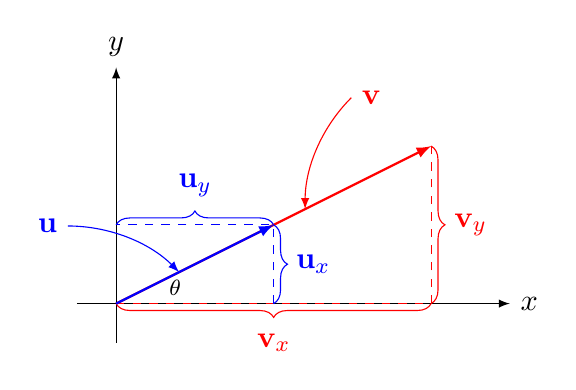
\begin{tikzpicture}
        \draw[black, -latex] (-0.5, 0) -- (5, 0) node[right] {$x$};
        \draw[black, -latex] (0, -0.5) -- (0, 3) node[above] {$y$};
        \draw[red, thick, -latex] (0, 0) -- (4, 2);
        \draw[red, thin, dashed] (0,0) -- (4, 0);
        \draw[red, thin, dashed] (4, 0) -- (4, 2);
        \draw[red, decorate, decoration = {brace, amplitude = 5pt, mirror}] 
        (0, 0) -- (4, 0) node[midway, yshift = -0.5cm] {$\textbf{v}_x$};
        \draw[red, decorate, decoration = {brace, amplitude = 5pt, mirror}] 
        (4, 0) -- (4, 2) node[midway, xshift = 0.5cm] {$\textbf{v}_y$};
        \draw[red, latex-] (2.4, 1.2) arc(180:135:2) node[right] {\textbf{v}};
        \draw[blue, thick, -latex] (0, 0) -- (2, 1);
        \draw[blue, latex-] (0.8, 0.4) arc(45:90:2) node[left] {\textbf{u}};
        \node[font = \footnotesize] at (0.75, 0.2) {$\theta$};
        \draw[blue, thin, dashed] (2, 0) -- (2, 1) -- (0, 1);
        \draw[blue, decorate, decoration = {brace, amplitude = 5pt, mirror}] 
        (2, 0) -- (2, 1) node[midway, xshift = 0.5cm] {$\textbf{u}_x$};
        \draw[blue, decorate, decoration = {brace, amplitude = 5pt}] 
        (0, 1) -- (2, 1) node[midway, yshift = 0.5cm] {$\textbf{u}_y$};
    \end{tikzpicture}
    \caption{\textbf{u} is a unit vector in the same direction as \textbf{v}}
    \label{fig:vector}
\end{figure}

We know that $\theta = \arctan{ \left( \textbf{v}_y / \textbf{v}_x \right)}$. 
Therefore, the $x$-component of the unit vector, \textbf{u}, is given by:
$$\textbf{u}_x = |\textbf{u}| \cos{ \theta} = \cos{ \left( \arctan{ \frac{
\textbf{v}_y}{\textbf{v}_x}} \right)}$$

Similarly, we know that:
$$\textbf{u}_y = |\textbf{u}| \sin{ \theta} = \sin{ \left( \arctan{ \frac{
\textbf{v}_y}{\textbf{v}_x}} \right)}$$

(Recall that since \textbf{u} is a unit vector, $|\textbf{u}| = 1$). 

Let's use this method to find a unit vector, \textbf{u}, in the same direction 
as $\textbf{v} = \left[ 2, 1 \right]$:
$$\textbf{u}_x = \cos{ \left( \arctan{ \frac{1}{2} } \right) } \approx \cos{ 
\left( 0.464 \right) } = \frac{2}{\sqrt{5}}$$
$$\textbf{u}_y = \sin{ \left( \arctan{ \frac{1}{2} } \right) } \approx \sin{ 
\left( 0.464 \right)} = \frac{1}{\sqrt{5}}$$

Therefore, a unit vector in the same direction as \textbf{v} is $\textbf{u} = 
\left[ 2/\sqrt{5}, 1/\sqrt{5} \right]$. 

And we can find the directional derivative:
$$D_{\textbf{u}}(x, y) = \textbf{u}_x \left[ \frac{\partial}{\partial x} f(x, 
y) \right] + \textbf{u}_y \left[ \frac{\partial}{\partial y} f(x, y) \right]$$
$$D_{\textbf{u}}(x, y) = \left( \frac{2}{\sqrt{5}} \right) \left[ \frac{
\partial}{\partial x} \left( 3x\sqrt{y} \right) \right] + \left( \frac{1}{
\sqrt{5}} \right) \left[ \frac{\partial}{\partial y} \left( 3x\sqrt{y} \right) 
\right]$$
$$D_{\textbf{u}}(x, y) = \left( \frac{2}{\sqrt{5}} \right) \left( 3\sqrt{y} 
\right) + \left( \frac{1}{\sqrt{5}} \right) \left( \frac{3x}{2\sqrt{y}} 
\right)$$
$$D_{\textbf{u}}(x, y) = \frac{12y + 3x}{2\sqrt{5y}}$$

To find the magnitude of the directional derivative at $(1, 4)$, we 
substitute for $x$ and $y$:
$$D_{\textbf{u}}(1, 4) = \frac{12(4) + 3(1)}{2\sqrt{5(4)}} = \frac{51}{4\sqrt{5}} 
\approx 5.702$$

\subsection{Unit Vectors in Higher Dimensions}
The trigonometric explanation for finding unit vectors is more difficult to 
visualize in higher dimensions. However, there is another method that works 
well in 2, 3, and higher dimensions. Recall that the magnitude of a vector, 
$\textbf{v} = \left[ \textbf{v}_x, \textbf{v}_y \right]$ is given by $| 
\textbf{v} | = \sqrt{\left( \textbf{v}_x \right)^2 + \left( \textbf{v}_y 
\right)^2}$. For a vector with $n$ dimensions, $\textbf{v} = \left[ \textbf{v}_
1, \textbf{v}_2, \cdots , \textbf{v}_n \right]$, the magnitude is given by $| 
\textbf{v} | = \sqrt{ \left( \textbf{v}_1 \right)^2 + \left( \textbf{v}_2 
\right)^2 + \cdots + \left( \textbf{v}_n \right)^2}$. 

To find a unit vector, \textbf{u}, in the same direction as \textbf{v}, we can 
scale \textbf{v} up or down so that its magnitude is 1. We can do this by 
dividing by \textbf{v}'s magnitude. Consider the two-dimensional vector used 
in the last example, $\textbf{v} = \left[ 2, 1 \right]$. Its magnitude is:
$$| \textbf{v} | = \sqrt{\left( 2 \right)^2 + \left( 1 \right)^2} = \sqrt{5}$$

Let's check if $\textbf{v} / | \textbf{v} |$ is a unit vector:
$$ \frac{\textbf{v}}{|\textbf{v}|} = \left( \frac{1}{\sqrt{5}} \right) \left[ 
2, 1 \right] = \left[ \frac{2}{\sqrt{5}}, \frac{1}{\sqrt{5}} \right]$$

And the magnitude of this scaled vector is:
$$ \left| \frac{\textbf{v}}{| \textbf{v} |} \right| = \sqrt{\left( \frac{2}{
\sqrt{5}} \right)^2 + \left( \frac{1}{\sqrt{5}} \right)^2} = \sqrt{\frac{4}{5} 
+ \frac{1}{5}} = \sqrt{1} = 1$$

Notice our unit vector is the same as we found using the trigonometric method 
above. 

<<<<<<< HEAD
Another way to think of the question is: what factor, $k$, can we multiply 
\textbf{v} by to yield a vector with a magnitude of 1? Let's see this method 
for the 3-dimensional vector $\textbf{v} = \left[ 3, 2, 1 \right]$. We are 
looking for a $k$ such that:
=======
Another way to think of the question is: What factor, $k$, can we multiply \textbf{v} by to yield a vector with a magnitude of 1? Let's see this method for the 3-dimensional vector $\textbf{v} = \left[ 3, 2, 1 \right]$. We are looking for a $k$ such that:
>>>>>>> 75c26aca4245f06f19f767709f3697abe6d41eba
$$|k\textbf{v}| = 1$$
$$|k \textbf{v}| = \left| \left[ 3k, 2k, 1k \right] \right| = \sqrt{\left( 3k 
\right)^2 + \left( 2k \right)^2 + \left( 1k \right)^2}$$
$$= \sqrt{9k^2 + 4k^2 + k^2} = k\sqrt{14} = 1$$

<<<<<<< HEAD
Which implies that $k = 1/\sqrt{14}$, which is $1/|\textbf{v}|$. And therefore 
a unit vector in the same direction as $\textbf{v} = \left[ 3, 2, 1 \right]$ 
is:
$$\textbf{u} = \frac{1}{\sqrt{14}} \left[ 3, 2, 1 \right] = \left[ \frac{3}{
\sqrt{14}}, \frac{2}{\sqrt{14}}, \frac{1}{\sqrt{14}} \right]$$
=======
Which implies that $k = 1/\sqrt{14}$, which is $1/|\textbf{v}|$. Therefore, a unit vector in the same direction as $\textbf{v} = \left[ 3, 2, 1 \right]$ is:
$$\textbf{u} = \frac{1}{\sqrt{14}} \left[ 3, 2, 1 \right] = \left[ \frac{3}{\sqrt{14}}, \frac{2}{\sqrt{14}}, \frac{1}{\sqrt{14}} \right]$$
>>>>>>> 75c26aca4245f06f19f767709f3697abe6d41eba


\begin{Exercise}[title = {Finding Directional Derivatives}, label = direction]
Find the directional derivative of the function at the given point in the 
direction of the given vector. 
\begin{enumerate}
    \item $f(x, y) = e^{3x} \sin{2y}$, $(0, \pi/6)$, $\textbf{v} = \left[ -3, 
    4 \right]$
    \item $f(x, y) = x^2y + xy^3$, $(2, 4)$, $\textbf{v} = 2 \textbf{i} - 
    \textbf{j}$
    \item $f(x, y, z) = \ln{ \left( x^2 + 3y - z \right)}$, $(2, 2, 1)$, 
    $\textbf{v} = \left[ 1, 1, 1 \right]$
\end{enumerate}
\vspace{100mm}
\end{Exercise}

\begin{Answer}[ref = direction]
\begin{enumerate}
    \item First, we define \textbf{u} such that $|\textbf{u}| = 1$ and 
    \textbf{u} is in the same direction as \textbf{v}:
    $$\textbf{u} = k \textbf{v} = \left[ -3k, -4k \right]$$
    $$\sqrt{ \left( -3k \right)^2 + \left( 4k \right)^2} = 1$$
    $$\sqrt{9k^2 + 16k^2} = \sqrt{25k^2} = 5k = 1$$
    $$k = \frac{1}{5}$$

    Therefore, we define $\textbf{u} = \left[ -3/5, 4/5 \right]$ and the 
    directional derivative is given by:
    $$D_u(x, y) = \left( \frac{-3}{5} \right) \frac{\partial}{\partial x} f(x, 
    y) + \left( \frac{4}{5} \right) \frac{\partial}{\partial y} f(x, y)$$
    $$= \left( \frac{-3}{5} \right) \frac{\partial}{\partial x} \left[ e^{3x} 
    \sin{2y} \right] + \left( \frac{4}{5} \right) \frac{\partial}{\partial y} 
    \left[ e^{3x} \sin{2y} \right]$$
    $$= \left( \frac{-3}{5} \right) \left( 3e^{3x} \sin{2y} \right) + \left( 
    \frac{4}{5} \right) \left( 2e^{3x} \cos{2y} \right)$$

    And substituting for $(x, y) = (0, \pi/6)$:
    $$D_u(0, \pi/6) = \left( \frac{-3}{5} \right) \cdot \left[ 3e^{3 \cdot 0} 
    \sin{ \left( \frac{\pi}{3} \right)} \right] + \left( \frac{4}{5} \right) 
    \cdot \left[ 2e^{3 \cdot 0} \cos{ \left( \frac{\pi}{3} \right)} \right]$$
    $$D_u(0, \pi/6) = \left( \frac{-3}{5} \right) \cdot \left[ 3 \cdot \frac{
    \sqrt{3}}{2} \right] + \left( \frac{4}{5} \right) \cdot \left[ 2 \cdot 
    \frac{1}{2} \right]$$
    $$d_u(0, \pi/6) = \left( \frac{-3}{5} \right) \cdot \left( \frac{3
    \sqrt{3}}{2} \right) + \left( \frac{4}{5} \right) \cdot \left( 1 \right)$$
    $$D_u(0, \pi/6) = \frac{-9\sqrt{3}}{10} + \frac{8}{10} = \frac{8-9\sqrt{3}
    }{10} \approx -0.759$$

    \item We can express \textbf{v} as $\textbf{v} = \left[ 2, -1 \right]$. 
    And we define \textbf{u} such that $| \textbf{u} | = 1$ and \textbf{u} is 
    in the same direction as \textbf{v}:
    $$\textbf{u} = k\textbf{v} = \left[ 2k, -k \right]$$
    $$\sqrt{\left( 2k \right)^2 + \left( -k \right)^2} = 1$$
    $$\sqrt{4k^2 + k^2} = \sqrt{5}k = 1$$
    $$k = \frac{1}{\sqrt{5}} = \frac{\sqrt{5}}{5}$$

    Therefore, we define $\textbf{u} = \left[ 2\sqrt{5}/5, -\sqrt{5}/5 \right]$
    and the directional derivative is given by:
    $$D_u(x, y) = \left( \frac{2\sqrt{5}}{5} \right) \frac{\partial}{\partial 
    x}f(x, y) + \left( \frac{-\sqrt{5}}{5} \right) \frac{\partial}{\partial y}
    f(x, y)$$
    $$= \left( \frac{2\sqrt{5}}{5} \right) \frac{\partial}{\partial x} \left[ 
    x^2y + xy^3 \right] + \left( \frac{-\sqrt{5}}{5} \right) \frac{\partial}{
    \partial y} \left[ x^2y + xy^3 \right]$$
    $$= \left( \frac{2\sqrt{5}}{5} \right) \left[ 2xy + y^3 \right] + \left( 
    \frac{-\sqrt{5}}{5} \right) \left[ x^2 + 3xy^2 \right]$$

    And substituting $(x, y) = (2, 4)$:
    $$D_u(2, 4) = \left( \frac{2\sqrt{5}}{5} \right) \left[ 2(2)(4) + 4^3 
    \right] + \left( \frac{-\sqrt{5}}{5} \right) \left[ 2^2 + 3(2)(4^2) 
    \right]$$
    $$D_u(2, 4) = \left( \frac{2\sqrt{5}}{5} \right) \left[ 80 \right] + \left(
    \frac{-\sqrt{5}}{5} \right) \left[ 100 \right]$$
    $$D_u(2, 4) = 32\sqrt{5} - 20\sqrt{5} = 12\sqrt{5} \approx 26.833$$

    \item We define \textbf{u} such that $| \textbf{u} | = 1$ and \textbf{u} 
    is in the same direction as \textbf{v}:
    $$\textbf{u} = k\textbf{v} = \left[k, k, k \right]$$
    $$\sqrt{k^2 + k^2 + k^2} = 1$$
    $$\sqrt{3}k = 1$$
    $$k = \frac{1}{\sqrt{3}} = \frac{\sqrt{3}}{3}$$

    Therefore, we let $\textbf{u} = \left[ \sqrt{3}/3, \sqrt{3}/3, \sqrt{3}/3 
    \right]$ and the directional derivative is given by:
    $$D_u(x, y, z) = \left( \frac{\sqrt{3}}{3} \right) \frac{\partial}{
    \partial x} f(x, y, z) + \left( \frac{\sqrt{3}}{3} \right) \frac{
    \partial}{\partial y}f(x, y, z) + \left( \frac{\sqrt{3}}{3} \right) 
    \frac{\partial}{\partial z} f(x, y, z)$$
    $$= \left( \frac{\sqrt{3}}{3} \right) \left[ \frac{\partial}{\partial x} 
    \ln{ \left( x^2 + 3y - z \right)} + \frac{\partial}{\partial y} \ln{ 
    \left( x^2 + 3y - z \right)} + \frac{\partial}{\partial z} \ln{ \left( 
    x^2 + 3y - z \right)} \right]$$
    $$= \left( \frac{\sqrt{3}}{3} \right) \left[ \frac{2x}{x^2 + 3y - z} + 
    \frac{3}{x^2 + 3y - z} + \frac{-1}{x^2 + 3y - z} \right]$$
    $$= \left( \frac{\sqrt{3}}{3} \right) \left[ \frac{2x + 2}{x^2 + 3y - z} 
    \right] = \frac{\sqrt{3} \left( 2x + 2 \right)}{3 \left( x^2 + 3y - z 
    \right)}$$

    And substituting $(x, y, z) = (2, 2, 1)$:
    $$D_u(2, 2, 1) = \frac{\sqrt{3} \left( 2(2) + 2 \right)}{3 \left( 2^2 + 
    3(2) - 1 \right)} = \frac{\sqrt{3} \left( 6 \right)}{3 \left( 9 \right)} 
    = \frac{2\sqrt{3}}{9} \approx 0.385$$
\end{enumerate}
\end{Answer}

\subsection{Maximizing the Gradient}
The directional derivative can be written as the dot product of two vectors:
$$D_u f(x, y) = af_x(x, y) + bf_y(x, y) = \left[ f_x(x, y), f_y(x, y) \right] 
\cdot \textbf{u}$$

<<<<<<< HEAD
The first vector, $\left[ f_x(x, y), f_y(x, y) \right]$, is called \textit{the 
gradient of f}\index{gradient}, and is noted as $\nabla f$. 
=======
The first vector, $\left[ f_x(x, y), f_y(x, y) \right]$ is called \textit{the 
gradient of f}\index{gradient} and is noted as $\nabla f$. The gradient 
operator, $\nabla$, is the derivative of a scalar function that results in a 
vector which shows the magnitude and direction of the greatest rate of change. 
>>>>>>> eabbbcc8b878e818b0fd1aeab6d3a95ed058f052

\begin{mdframed}[style = important, frametitle = {The Gradient}]
For a two-variable function, $f(x, y)$, the gradient of $f$ is the vector:
$$\nabla f = \left[ f_x(x, y), f_y(x, y) \right] = \frac{\partial f}{\partial 
x} \textbf{i} + \frac{\partial f}{\partial y} \textbf{j}$$

Where \textbf{i} and \textbf{j} are the unit vectors in the $x$- and 
$y$-directions, respectively.
\end{mdframed}

Think back to the elevation example we opened the chapter with. What if we 
wanted to complete our ascent as quickly as possible? We would want to 
know the direction in which the elevation is changing the fastest. This occurs 
when the direction we are going is the same direction as the gradient vector, 
$\nabla f$. 

Recall that the dot product is defined as:
$$\textbf{u} \cdot \textbf{v} = \left| \textbf{u} \right| \left| \textbf{v} 
\right| \cos{ \theta}$$

Where $\theta$ is the angle between the vectors \textbf{u} and \textbf{v}. 
Applying this to the directional derivative, we see that:
$$D_u f = \nabla f \cdot \textbf{u} = \left| \nabla f \right| \left| 
\textbf{u} \right| \cos{\theta} = \left| \nabla f \right| \cos{\theta}$$

Which is at its maximum when $\nabla f$ and \textbf{u} point in the same 
direction (because $\cos{\left( 0 \right)} = 1$). Therefore, the gradient 
vector points in the direction of maximum change and the magnitude of that 
vector is the rate of maximum change. 

\textbf{Example}: Find the maximum rate of change of $f(x, y) = 4y\sqrt{x}$ at 
$(4, 1)$. In what direction does the maximum change occur?

\textbf{Solution}: We begin by finding $\nabla f$:
$$\nabla f = \left[ \frac{\partial}{\partial x} \left( 4y\sqrt{x} \right), 
\frac{\partial}{\partial y} \left( 4y\sqrt{x} \right) \right]$$
$$\nabla f = \left[ \frac{2y}{\sqrt{x}}, 4\sqrt{x} \right]$$

And thus, 
$$\nabla f(4, 1) = \left[ \frac{2(1)}{\sqrt{4}}, 4\sqrt{4} \right] = \left[ 1, 
8 \right]$$

Therefore, the maximum value of $\nabla f$ at $(4, 1)$ is:
$$\left| \nabla f \right| = \sqrt{1^2 + 8^2} = \sqrt{65}$$

in the direction of the vector $\left[ 1, 8 \right]$. 

\begin{Exercise}[title = {Using the Gradient to find Maximum Change}, 
label = maximum]
Suppose you are climbing a mountain whose elevation is described by $z = 3000 
- 0.01x^2 - 0.02y^2$. Take the positive $x$-direction to be east and the 
positive $y$-direction to be north. 
\begin{enumerate}
    \item If you are at $(x, y) = (50, 50)$, what is your elevation?
    \item If you walk south, will you ascend or descend?
    \item If you walk northwest, will you ascend or descend? Will the rate of 
    elevation change be greater or less than if you walked south?
    \item In what direction should you walk for the steepest ascent? What will 
    your ascension rate be?
\end{enumerate}
\vspace{50mm}
\end{Exercise}

\begin{Answer}[ref = maximum]
\begin{enumerate}
    \item $z = f(50, 50) = 3000 - 0.01(50)^2 - 0.02(50)^2 = 2925$
    \item A south-pointing unit vector is $\textbf{u} = \left[ 0, -1 \right]$. 
    To find the rate of change, we find the directional derivative in the 
    direction of \textbf{u} at $(50, 50)$:
    $$D_u f(x, y) = \left( -1 \right) \left[ \frac{\partial}{\partial y} 
    \left( 3000 - 0.01x^2 - 0.02y^2 \right) \right]$$
    $$D_u f(x, y) = \left( -1 \right) \left( -0.04 y \right) = 0.04y$$

    And at $(50, 50)$, $D_u f(50, 50) = 0.04(50) = 2 > 0$. Therefore, if you 
    walk south, you will ascend.
    \item A northwest-pointing unit vector is $\textbf{u} = \left[ -\sqrt{2}
    /2, \sqrt{2}/2 \right]$. To find the rate of change, we find the 
    directional derivative at $(50, 50)$ in the direction of \textbf{u}:
    $$D_u f(x, y) = \left( \frac{-\sqrt{2}}{2} \right) \left[ \frac{\partial}{
    \partial x} f(x, y) \right] + \left( \frac{\sqrt{2}}{2} \right) \left[ 
    \frac{\partial}{\partial y} f(x, y) \right]$$
    $$D_u f(x, y) = \left( \frac{-\sqrt{2}}{2} \right) \left[ -0.02x \right] 
    + \left( \frac{\sqrt{2}}{2} \right) \left[ -0.04 y \right]$$
    $$D_u f(x, y) = 0.01\sqrt{2}x - 0.02\sqrt{2}y$$
    $$D_u f(50, 50) = 0.01 \sqrt{2} \left( 50 \right) - 0.02 \sqrt{2} \left( 
    50 \right) = \frac{-\sqrt{2}}{2} \approx -0.707$$

    The rate of elevation change walking northwest is approximately $-0.707$, 
    so you will descend and your rate of elevation change would be less than 
    if you walked south. 

    \item To find the direction of maximum elevation gain, we find the 
    direction the gradient vector points in:
    $$\nabla f = \left[ \frac{\partial f}{\partial x}, \frac{\partial f}{
    \partial y} \right]$$
    $$\nabla f = \left[ -0.02x, -0.04y \right]$$

    And at $(50, 50)$, 
    $$\nabla f(50, 50) = \left[ -0.02(50), -0.04(50) \right] = \left[ -1, -2 
    \right]$$

    Therefore, the rate of greatest elevation change is in a south-by-southwest 
    direction indicated by the vector $\left[ -1, -2 \right]$ and the rate of 
    elevation change is $\left| \nabla f(50, 50) \right| = \sqrt{(-1)^2 + (-2)^
    2} = \sqrt{5}$. Notice this is greater than the other two rates of change 
    we have found. 
\end{enumerate}
\end{Answer}

\section{Applications of Partial Derivatives and Gradients}

\subsection{Laplace's Equation}
A partial differential equation that has applications in fluid dynamics and 
electronics is Laplace's equation\index{Laplace's equation}. Solutions to 
Laplace's equation are called \textit{harmonic functions}. 

\begin{mdframed}[style = important, frametitle = {Laplace's Equation}]
Consider a twice-differentiable function, $f$. In two dimensions, Laplace's 
Equation is given by:
$$ \frac{\partial ^2 f}{\partial x^2} + \frac{\partial^2 f}{\partial y^2} = 0$$
And in three dimensions, 
$$\frac{\partial ^2 f}{\partial x^2} + \frac{\partial ^2 f}{\partial y^2} + 
\frac{\partial ^2 f}{\partial z^2} = 0$$
\end{mdframed}

Another way to represent Laplace's equation is:
$$\delta f = \nabla^2 f = \nabla \cdot \nabla f = 0$$

Where $\nabla ^2 = \delta$ is called the \textit{Laplace operator}. 

\textbf{Example}: Determine whether or not $f = x^2 + y^2$ is a solution to 
Laplace's equation. 

\textbf{Solution}: We are checking to see if $\frac{\partial^2 f}{\partial 
x^2} + \frac{\partial^2 f}{\partial y^2} = 0$ for $f(x, y) = x^2 + y^2$. 
Finding $\partial^2 f / \partial x^2$:
$$\frac{\partial^2 f}{\partial x^2} = \frac{\partial}{\partial x} \left[ \frac{
\partial}{\partial x} \left( x^2 + y^2 \right) \right]$$
$$= \frac{\partial}{\partial x} \left( 2x \right) = 2$$

And finding $\partial^2 f / \partial y^2$:
$$\frac{\partial^2 f}{\partial y^2} = \frac{\partial}{\partial y} \left[ \frac{
\partial}{\partial y} \left( x^2 + y^2 \right) \right]$$
$$= \frac{\partial}{\partial y} \left( 2x \right) = 2$$

Then $\frac{\partial^2 f}{\partial x^2} + \frac{\partial^2 f}{\partial y^2} = 
2 + 2 = 4 \neq 0$. Therefore, $f(x, y) = x^2 + y^2$ is not a solution to 
Laplace's equation. 

\begin{Exercise}[title = {Solutions to Laplace's Equation}, label = laplace]
Determine whether the function is a solution to Laplace's equation. 
\begin{enumerate}
    \item $f(x, y) = x^2 - y^2$
    \item $f(x, y) = \sin{x} \cosh{y} + \cos{x} \sinh{y}$
    \item $f(x, y) = e^{-x} \cos{y} - e^{-y} \cos{x}$
\end{enumerate}
\vspace{50mm}
\end{Exercise}

\begin{Answer}[ref = laplace]
\begin{enumerate}
    \item $$\frac{\partial^2 f}{\partial x^2} + \frac{\partial^2 f}{\partial 
    y^2} = \frac{\partial}{\partial x} \left[ \frac{\partial}{\partial x} 
    \left( x^2 - y^2 \right) \right] + \frac{\partial}{\partial y} \left[ 
    \frac{\partial}{\partial y} \left( x^2 - y^2 \right) \right]$$
    $$= \frac{\partial}{\partial x} \left[ 2x \right] + \frac{\partial}{
    \partial y} \left[ -2y \right] = 2 - 2 = 0$$

    Therefore, $f(x, y) = x^2 - y^2$ is a solution to Laplace's equation. 

    \item $$\frac{\partial^2}{\partial x^2} + \frac{\partial^2}{\partial y^2} 
    = \frac{\partial}{\partial x} \left[ \frac{\partial}{\partial x} \left( 
    \sin{x} \cosh{y} + \cos{x} \sinh{y} \right) \right] + \frac{\partial}{
    \partial y} \left[ \frac{\partial}{\partial y} \left( \sin{x} \cosh{y} + 
    \cos{x} \sinh{y} \right) \right]$$
    $$= \frac{\partial}{\partial x} \left[ \cos{x} \cosh{y} - \sin{x} \sinh{y} 
    \right] + \frac{\partial}{\partial y} \left[ \sin{x} \sinh{y} + \cos{x} 
    \cosh{y} \right]$$
    $$= -\sin{x}\cosh{y} - \cos{x}\sinh{y} + \sin{x}\cosh{y} + \cos{x} \sinh{
    y} = 0$$

    Therefore, $f(x, y) = \sin{x}\cosh{y} + \cos{x}\sinh{y}$ is a solution to 
    Laplace's equation.

    \item $$\frac{\partial^2 f}{\partial x^2} + \frac{\partial^2 f}{\partial 
    y^2} = \frac{\partial}{\partial x} \left[ \frac{\partial}{\partial x} 
    \left( e^{-x}\cos{y} - e^{-y}\cos{x} \right) \right] + \frac{\partial}{
    \partial y} \left[ \frac{\partial}{\partial y} \left( e^{-x} \cos{y} - 
    e^{-y} \cos{x} \right) \right]$$
    $$= \frac{\partial}{\partial x} \left[ -e^{-x}\cos{y} + e^{-y}\sin{x} 
    \right] + \frac{\partial}{\partial y} \left[ -e^{-x}\sin{y} + e^{-y} 
    \cos{x} \right]$$
    $$= e^{-x} \cos{y} + e^{-y} \cos{x} - e^{-x} \cos{y} - e^{-y} \cos{x} = 0$$

    Therefore, $f(x, y) = e^{-x}\cos{y} - e^{-y}\cos{x}$.
\end{enumerate}
\end{Answer}

\subsection{The Wave Equation}
Another useful equation with partial derivatives is the Wave Equation:
$$\frac{\partial^2 f}{\partial t^2} = a^2 \frac{\partial^2 f}{\partial x^2}$$

Where $f$ is a function of $x$ and $t$ and $a$ is a constant. This equation 
describes waves, such as a vibrating string, light waves, or sound waves. 

\textbf{Example}: Show that $f(x, t) = \sin{ \left( x - at \right)}$ satisfies 
the wave equation. 

\textbf{Solution}: First, we find the second partial derivatives:
$$\frac{\partial^2 f}{\partial t^2} = \frac{\partial}{\partial t} \left[ \frac{
\partial}{\partial t} \left( \sin{ \left( x - at \right)} \right) \right] = 
\frac{\partial}{\partial t} \left[ -a\cos{\left(x - at \right)} \right] = -a^2
\sin{\left(x - at \right)}$$

$$\frac{\partial^2 f}{\partial x^2} = \frac{\partial}{\partial x} \left[ \frac{
\partial}{\partial x} \left( \sin{ \left( x - at \right)} \right) \right] = 
\frac{\partial}{\partial x} \left[ \cos{\left( x - at \right)}\right] = -\sin{
\left( x - at \right)}$$

And we see that:
$$a^2 \frac{\partial^2 f}{\partial x^2} = -a^2 \sin{\left(x - at \right)} = 
\frac{\partial^2 f}{\partial t^2}$$

Therefore, this function satisfies the wave equation. 

\begin{Exercise}[title = {The Wave Equation}, label = wave]
Show that the following functions satisfy the wave equation:
\begin{enumerate}
    \item $f(x, t) = \cos{\left(kx \right)}\cos{\left(akt \right)}$
    \item $f(x, t) = \sin{\left( x - at \right)} + \ln{ \left( x + at 
    \right)}$
    \item $f(x, t) = \frac{t}{a^2t^2 - x^2}$
\end{enumerate}
\vspace{50mm}
\end{Exercise}

\begin{Answer}[ref = wave]
\begin{enumerate}
    \item Finding the partial derivatives:
    $$\frac{\partial^2 f}{\partial t^2} = \frac{\partial}{\partial t} \left[ 
    \frac{\partial}{\partial t} \left( \cos{ \left( k x \right)} \cos{ \left( 
    a k t \right)} \right) \right] = \frac{\partial}{\partial t} \left[ -a k 
    \cos{ \left( k x \right)} \sin{ \left( a k t \right)} \right]$$
    $$\frac{\partial^2 f}{\partial t^2} = -a^2 k^2 \cos{ \left( k x \right)} 
    \cos{ \left( a k t \right)}$$

    $$\frac{\partial^2 f}{\partial x^2} = \frac{\partial}{\partial x} \left[ 
    \frac{\partial}{\partial x} \left( \cos{\left( k x \right)}\cos{\left( a k 
    t \right)} \right) \right] = \frac{\partial}{\partial x} \left[ -k \sin{ 
    \left( k x \right)} \cos{ \left( a k t \right)} \right]$$
    $$\frac{\partial^2 f}{\partial x^2} = -k^2 \cos{ \left( k x \right)} \cos{ 
    \left( a k t \right)}$$

    And we see that:
    $$a^2 \frac{\partial^2 f}{\partial x^2} = -a^2 k^2 \cos{ \left( k x 
    \right)} \cos{ \left( a k t \right)} = \frac{\partial^2 f}{\partial t^2}$$

    Therefore, $f(x, t) = \cos{\left( k x \right)}\cos{\left( a k t \right)}$ 
    satisfies the wave equation. 

    \item Finding the partial derivatives:
    $$\frac{\partial^2 f}{\partial t^2} = \frac{\partial}{\partial t} \left[ 
    \frac{\partial}{\partial t} \left( \sin{\left( x - a t \right)} + \ln{ 
    \left( x + a t \right)} \right) \right]$$
    $$\frac{\partial^2 f}{\partial t^2} = \frac{\partial}{\partial t} \left[ 
    -a \cos{ \left( x - a t \right)} + \frac{a}{x + a t} \right] = -a^2 \sin{ 
    \left( x - a t \right)} + \frac{-a^2}{\left( x + a t \right)^2}$$

    $$\frac{\partial^2 f}{\partial x^2} = \frac{\partial}{\partial x} \left[ 
    \frac{\partial}{\partial x} \left( \sin{ \left( x - a t \right)} + \ln{ 
    \left( x + a t \right)} \right) \right]$$

    $$\frac{\partial^2 f}{\partial x^2} = \frac{\partial}{\partial x} \left[ 
    \cos{ \left( x - a t \right)} + \frac{1}{x + a t} \right] = -\sin{ \left( 
    x - a t \right)} + \frac{-1}{\left( x + a t \right)^2}$$

    And we see that:
    $$a^2 \frac{\partial^2 f}{\partial x^2} = -a^2 \sin{ \left( x - a t 
    \right)} + \frac{-a^2}{\left( x + a t \right)^2} = \frac{\partial^2 f}{
    \partial t^2}$$

    Therefore, $f(x, t) = \sin{ \left( x - a t \right)} + \ln{ \left( x + a t 
    \right)}$ satisfies the wave equation. 

    \item Finding the partial derivatives:
    $$\frac{\partial^2 f}{\partial t^2} = \frac{\partial}{\partial t} \left[ 
    \frac{\partial}{\partial t} \left( \frac{t}{a^2 t^2 - x^2} \right) \right] 
    = \frac{\partial}{\partial t} \left[ \frac{\left(a^2 t^2 - x^2 \right) - t 
    \left(2 a^2 t \right)}{\left( a^2 t^2 - x^2 \right)^2} \right]$$
    $$\frac{\partial^2 f}{\partial t^2} = \frac{\partial}{\partial t} \left[ 
    \frac{a^2 t^2 - x^2 - 2 a^2 t^2}{\left( a^2 t^2 - x^2 \right)^2} \right] = 
    \frac{\partial}{\partial t} \left[ \frac{-a^2 t^2 - x^2}{\left( a^2 t^2 - 
    x^2 \right)^2} \right]$$
    $$\frac{\partial^2 f}{\partial t^2} = \frac{\left( a^2 t^2 - x^2 \right)^2 
    \left(-2 a^2t \right) - \left( -a^2 t^2 - x^2 \right) \left( 2 \left( a^2 
    t^2 - x^2 \right) \left( 2 a^2 t \right) \right)}{\left( a^2 t^2 - x^2 
    \right)^4}$$
    $$\frac{\partial^2 f}{\partial t^2} = \frac{\left( a^2 t^2 - x^2 \right) 
    \left( -2 a^2 t \right) - \left( -a^2 t^2 - x^2 \right) \left( 4 a^2 t 
    \right)}{\left( a^2 t^2 - x^2 \right)^3}$$
    $$\frac{\partial^2 f}{\partial t^2} = \frac{ -2 a^4 t^3 + 2 a^2 t x^2 + 4 
    a^4 t^3 + 4 a^2  t x^2}{\left( a^2 t^2 - x^2 \right)^3}$$
    $$\frac{\partial^2 f}{\partial t^2} = \frac{ 2 a^4 t^3 + 6 a^2 t x^2}{
    \left( a^2 t^2 - x^2 \right)^3} = 2 a^2 t \left( \frac{a^2 t^2 + 3 x^2}{
    \left( a^2 t^2 - x^2 \right)^3} \right)$$

    $$\frac{\partial^2 f}{\partial x^2} = \frac{\partial}{\partial x} \left[ 
    \frac{\partial}{\partial x} \left( \frac{t}{a^2 t^2 - x^2} \right) \right] 
    = \frac{\partial}{\partial x} \left[ \frac{\left( a^2 t^2 - x^2 \right) 
    \left( 0 \right) - t \left( -2 x \right)}{\left( a^2  t^2 - x^2 \right)^2} 
    \right]$$
    $$\frac{\partial^2 f}{\partial x^2} = \frac{\partial}{\partial x} \left[ 
    \frac{2 t x}{\left( a^2 t^2 - x^2 \right)^2} \right] = \frac{\left( a^2 
    t^2 - x^2 \right)^2 \left( 2 t \right) - \left( 2 t x \right) \left( 2 
    \left( a^2 t^2 - x^2 \right) \left( -2 x \right) \right)}{\left( a^2 t^2 - 
    x^2 \right)^4}$$
    $$\frac{\partial^2 f}{\partial x^2} = \frac{\left( a^2 t^2 - x^2 \right) 
    \left( 2 t \right) - \left( 2 t x \right) \left( 2 \right) \left( -2 x 
    \right)}{\left( a^2 t^2 - x^2 \right)^3}$$
    $$\frac{\partial^2 f}{\partial x^2} = \frac{2 a^2 t^3 - 2 t x^2 + 8 t x^2}{
    \left( a^2 t^2 - x^2 \right)^3} = \frac{2 a^2 t^3 + 6 t x^2}{\left( a^2 
    t^2 - x^2 \right)^3} = 2 t \left( \frac{a^2 t^2 + 3 x^2}{\left( a^2 t^2 - 
    x^2 \right)^3} \right)$$

    And we see that:
    $$a^2 \frac{\partial^2 f}{\partial x^2} = 2 a^2 t \left( \frac{a^2 t^2 + 3 
    x^2}{\left( a^2 t^2 - x^2 \right)^3} \right) = \frac{\partial^2 f}{
    \partial t^2}$$

    Therefore, $f(x, t) = \frac{t}{a^2t^2 - x^2}$ satisfies the wave equation. 
\end{enumerate}
\end{Answer}

\subsection{Cobb-Douglas Production Function}
The Cobb-Douglas function describes the marginal utility of capital and labor 
as theorized by the economists Charles Cobb and Paul Douglas. Capital 
investments are things like new machinery, expanded factories, or raw 
materials. Labor investments involve hiring more workers or improving 
working conditions to improve work rates. We can describe total production, 
$P$, as a function of labor, $L$, and capital, $K$. Cobb and Douglas posit 
three conditions:
\begin{enumerate}
\item Without either labor or capital, production will cease.
\item The marginal utility of labor is proportional to the amount of production 
per unit of labor.
\item The marginal utility of capital is proportional to the amount of 
production per unit of capital.
\end{enumerate}

The marginal utility of labor is given by the partial derivative, $\partial P 
/ \partial L$ and the production per unit of labor is given by $P / L$. 
Therefore, statement 2 says that:
$$\frac{\partial P}{\partial L} = \alpha \frac{P}{L}$$

where $\alpha$ is some constant. Keeping $K$ constant at $K = K_0$, we have 
the differential equation:
$$ \frac{d P}{d L} = \alpha \frac{P}{L}$$

Solving, we find that:
$$P(L, K_0) = C_1 \left( K_0 \right) L^{\alpha}$$

We make $C_1$ a function of $K_0$ because it could depend on $K_0$. In a 
similar manner to above, we can write statement 3 as a mathematical statement:
$$\frac{\partial P}{\partial K} = \beta \frac{P}{K}$$

where $\beta$ is also a constant. Keeping $L = L_0$ and solving, we see that:
$$P(L_0, K) = C_2(L_0)K^{\beta}$$

again, we assume $C_2$ is a function of the fixed labor, $L_0$. Combining 
these equations, we get:
$$P(L, K) = bL^{\alpha} K^{\beta}$$

where $b$ is a constant independent of capital and labor. Additionally, from 
statement 1, we know that $\alpha > 0$ and $\beta > 0$. What happens if both 
labor and capital are increased by a factor of $n$? Let's examine the effect 
on $P$:
$$P(nL, nK) = b \left( nL \right)^{\alpha} \left( nK \right)^{\beta}$$
$$P(nL, nK) = n^{\alpha + \beta} b L^{\alpha} K^{beta} = n^{\alpha + \beta} 
P(L, K)$$

Cobb and Douglas noted that if $\alpha + \beta = 1$, then $P(nL, nK) = nP(L, 
K)$, and therefore increasing labor and capital by a factor of $n$ increases 
production by a factor of $n$ as well. Therefore, the Cobb-Douglas equation 
assumes $\alpha + \beta = 1$ and can be written as:
$$P(L, K) = bL^{\alpha}K^{1 - \alpha}$$

\begin{Exercise}[title = {Cobb-Douglas Production Model}, label = cobb]
Cobb and Douglas modeled production in the US from 1900 to 1922 with the 
equation $P(L, K) = 1.01L^{0.75} K^{0.75}$. 
\begin{enumerate}
\item Express the marginal utility of labor as a function of $L$ and $K$.
\item Express the marginal utility of capital as a function of $L$ and $K$.
\item In 1916, $L = 382$ and $K = 126$ (compared to initial values of $100$ in 
1900). What is the marginal utility of labor in 1916? Of capital?
\item Based on your answer to the previous question, would you invest in 
capital or labor if you owned a factory in 1916? Why?
\end{enumerate}
\vspace{50mm}
\end{Exercise}

\begin{Answer}[ref = cobb]
\begin{enumerate}
    \item The marginal utility of labor is given by $\partial P / \partial L$:
    $$\frac{\partial P}{\partial L} = \frac{\partial}{\partial L} \left[ 1.01 
    L^{0.75} K^{0.25} \right] = 0.7575 L^{-0.25} K^{0.25}$$
    \item The marginal utility of capital is given by $\partial P / \partial 
    K$:
    $$\frac{\partial P}{\partial K} = \frac{\partial}{\partial K} \left[ 1.01 
    L^{0.75} K^{0.25} \right] = 0.2525 L^{0.75} K^{-0.75}$$
    \item Finding the marginal utility of labor in 1916:
    $$\frac{\partial P}{\partial L} = 0.7575 \left( 382 \right)^{-.25} \left( 
    126 \right)^{0.25} \approx 0.574$$
    And finding the marginal utility of capital in 1916:
    $$\frac{\partial P}{\partial K} = 0.2525 \left( 382 \right)^{0.75} \left( 
    126 \right)^{-0.75} \approx 0.580$$
    \item Since the marginal utility of capital is greater, I would invest in 
    capital. This would yield a greater increase in production than the same 
    investment in labor. 
\end{enumerate}
\end{Answer}
%%%%%%%%%%%%%%%%%%%%%%%%%%%%%%%%%
%% Bookfooter.tex by Aaron Hillegass
%% Nov 8, 2020

\appendix

\chapter{Answers to Exercises}
\shipoutAnswer

\bibliography{references}

\printindex

\end{document}